% ============================================================
%  ch6_experimental_evaluation.tex
%  Chapter 6: Experimental Evaluation
%  Master's Thesis -- SQL MATCH_RECOGNIZE on Pandas DataFrames
% ============================================================
% !TEX root = Thesis.tex
\chapter{Experimental Evaluation}
\label{chap:evaluation}

This chapter evaluates the implementation on five criteria:
correctness against Trino and Oracle, SQL:2016 feature coverage,
performance, scalability, and usability.
Section~\ref{sec:eval-methodology} defines the methodology,
Section~\ref{sec:eval-dataset} the datasets and patterns,
Section~\ref{sec:eval-correctness} validates the concept example by
example, Section~\ref{sec:eval-coverage} reports coverage and
complexity results, and Section~\ref{sec:eval-performance} presents
the cross-system performance analysis.

% ----------------------------------------------------------------
\section{Evaluation Methodology}
\label{sec:eval-methodology}
% ----------------------------------------------------------------

Section~\ref{subsec:eval-metrics} defines the five criteria and how
each is measured; Section~\ref{subsec:eval-environment} describes the
hardware and software environment.

% ................................
\subsection{Evaluation Criteria and Metrics}
\label{subsec:eval-metrics}
% ................................

\paragraph{Correctness.}
The result DataFrame is compared against two independent SQL
references, Trino~473 and Oracle~21c EE, by exact row-level equality
(same rows, values, and order where deterministic).  This covers the
two small synthetic tables introduced in
Section~\ref{sec:eval-dataset}, \texttt{orders} and
\texttt{stock\_price}, and the 30 pattern--size combinations of the
Amazon benchmark: five pattern families run at each of six sizes, so
30 cells per system and 90 in total.  Each of the two tables has three
columns: a key that partitions the rows, a date that orders them, and a
price the pattern tests (Figure~\ref{fig:eval-sample-tables}).  The SQL
engines are the
correctness references.  The hand-written Pandas functions provide an
additional output cross-check and the usability baseline
(Section~\ref{subsec:eval-usability}).

\begin{figure}[htbp]
  \centering
  \begin{tikzpicture}[
      tbl/.style={draw=black!55, rounded corners=2pt, inner sep=5pt,
                  align=left, font=\footnotesize},
      note/.style={font=\footnotesize, text=black!70}]
    \node[tbl] (orders) {\textbf{\texttt{orders}}\\[3pt]
      \begin{tabular}{@{}ll@{}}
        \texttt{customer\_id} & $\rightarrow$ \texttt{PARTITION BY}\\
        \texttt{order\_date}  & $\rightarrow$ \texttt{ORDER BY}\\
        \texttt{price}        & $\rightarrow$ \texttt{DEFINE}
      \end{tabular}};
    \node[tbl, right=10mm of orders] (stock)
      {\textbf{\texttt{stock\_price}}\\[3pt]
      \begin{tabular}{@{}ll@{}}
        \texttt{Company}     & $\rightarrow$ \texttt{PARTITION BY}\\
        \texttt{Price\_date} & $\rightarrow$ \texttt{ORDER BY}\\
        \texttt{Price}       & $\rightarrow$ \texttt{DEFINE}
      \end{tabular}};
    \node[note, below=3pt of orders] {Example~1};
    \node[note, below=3pt of stock] {Examples~2 and~3};
  \end{tikzpicture}
  \caption[Columns of the two synthetic tables]{Columns of the two
    synthetic tables and the clause that uses each one.  The tables are
    independent; each serves its own worked examples.}
  \label{fig:eval-sample-tables}
\end{figure}

\paragraph{SQL feature coverage.}
Two views are recorded, both reported in
Section~\ref{sec:eval-coverage}.  The same boundary is written up for
users in the package guide, which gives a status table for the main
clauses and pattern constructs, names what is not supported, and lists
the errors the API raises~\cite{monierashraf2025guide}.  \emph{Feature coverage} marks each
main \texttt{MATCH\_RECOGNIZE} clause as \emph{supported},
\emph{partially supported}, or \emph{unsupported} against the
reference tests.  The clauses are
partitioning, ordering, \texttt{PATTERN}, \texttt{DEFINE},
\texttt{MEASURES}, \texttt{SUBSET}, the output and skip modes, and
navigation
functions~\cite{iso2016,ISO2021,monierashraf2025rowmatch}.
\emph{Pattern-type coverage} groups the test cases by row-pattern
type (simple sequences, quantified repetitions, trends, recovery,
alternation, exclusions, anchors, and \texttt{PERMUTE}); a type is
covered when at least one case matches the reference output.

\paragraph{Performance.}
Execution time is the client-observed end-to-end latency per
pattern--size run on the Amazon UK Products dataset
(Section~\ref{subsec:eval-real-dataset}): five pattern families, six
sizes, result transfer included.  Each cell runs five warmups, then
twenty measured runs, each preceded by a five-second idle window that
sets the pre-query memory baseline.

The warmups matter because a first run measures start-up rather than
steady state.  Trino runs on the Java Virtual Machine (JVM), which
compiles its own bytecode
to machine code while the early queries execute; that
\emph{just-in-time} (JIT) step makes them slower than later runs.
Oracle fills its caches, and the engine compiles the pattern once.

Outliers are then removed per metric with the $1.5\times$ interquartile
range (IQR) rule: the IQR is the spread between the 25th and 75th
percentiles, and a run lying more than $1.5\times$ that spread outside
them is dropped.  It discarded 99 of the 1{,}800 measured time runs.
Cells report the mean of the retained runs with its standard deviation.
Throughput is computed per run, as dataset size divided by that run's
time, and then averaged the same way, so it is the mean of the rates
rather than the rate of the mean.  The two differ because a rate is one
over a time, and averaging that inverse gives a slow run less weight;
over the main matrix the gap is $0.12$\% or less.  For the main
benchmark, the two
memory metrics use one instrument for all three systems.
\emph{Query memory} is the rise above the idle baseline while the query
runs, and \emph{footprint memory} is the highest total the process or
container reaches.  Their scope is defined in
Section~\ref{subsec:eval-memory}.

\paragraph{Scalability.}
For each pattern family, the cell means are fitted with a straight
line against row count by least squares.  The fit is summarised by
$R^2$, the share of the variation in measured time that the line
accounts for, where $1$ is a perfect fit.  It is reported for both the
six-size benchmark and the larger stress test.  A high $R^2$ describes
the measured range only.  It does not prove the algorithm's asymptotic
complexity, because over a range this narrow an $O(n \log n)$ cost is
itself close to straight
(Section~\ref{subsec:eval-complexity}).

\paragraph{Usability (developer effort).}
For each worked example, the line count of the idiomatic Pandas
solution is compared with the single \texttt{MATCH\_RECOGNIZE}
statement in Section~\ref{subsec:eval-usability}, counting only the
detection logic on both sides.  Line count is a proxy for developer
effort rather than a measurement of it.  It reflects how much
procedural detail the author must write and later maintain, and says
nothing about reading time, error rate, or learning
cost~\cite{iso2016,ISO2021,melton2017sqlrpr,Python_UDF}.

% ................................
\subsection{Environment and Configuration}
\label{subsec:eval-environment}
% ................................

The experiments ran on a workstation with an Intel Core i7-11800H
processor and 64\,GB of RAM under Ubuntu 24.04.4 LTS.  For the
cross-system benchmark, each system had the same outer control-group
limit of one CPU core and 32\,GB.
Section~\ref{subsec:eval-pattern-defs} details the
enforcement mechanisms.

The scalability stress test (Section~\ref{subsec:eval-stress}) instead
uses a 58\,GB memory limit.  Reaching hundreds of millions of rows on equal
terms also meant changing the Trino deployment: it reads from a
disk-backed Hive/Parquet connector rather than its in-memory
connector.  All database containers run on the
host's native Docker daemon, so container limits map directly to host
control groups.  A control group, or \emph{cgroup}, is the Linux kernel
facility that caps and reports the CPU and memory of a set of
processes, and it is the same instrument used for the engine.

The software stack comprised the two baseline SQL engines, Trino~473 and
Oracle~21c EE, each run as a Docker container.  It also included the
Java~11.0.25 LTS and Python~3.12.7 runtimes and the core Python
libraries \texttt{pandas}~2.3.3, \texttt{numpy}~2.1.3,
\texttt{antlr4-python3-\allowbreak{}runtime}~4.13.2,
\texttt{antlr4-\allowbreak{}tools}~0.2.1, and \texttt{pytest}~8.3.4.
The implementation itself uses ANTLR4 to parse Trino SQL,
Pandas for DataFrame management, and custom AST/NFA/DFA
modules for pattern detection (Chapter~\ref{chap:methodology}).

Unless stated otherwise, all experiments use this configuration.
For correctness comparisons, identical data are loaded into all three
systems and result sets are compared by row order and measure values
(after normalizing case-only column-name differences).

% ----------------------------------------------------------------
\section{Dataset and Test Patterns}
\label{sec:eval-dataset}
% ----------------------------------------------------------------

\label{subsec:eval-dataset-orders}

Four datasets are used.  Two are small synthetic tables that can be
verified by hand, \texttt{orders} and \texttt{stock\_price}
(Figure~\ref{fig:eval-sample-tables}).  The
real-world Amazon UK Products dataset, up to 2.2\,million rows, carries
the cross-system timing and memory benchmark.  The Amazon Reviews~2023
corpus, up to 227.9\,million rows, carries the scalability test
(Section~\ref{subsec:eval-stress}).

\paragraph{Dataset 1: the \texttt{orders} table.}
The \texttt{orders} table supports the first worked example.  It
comprises three attributes~\cite{trino2021row}: \texttt{customer\_id}
(\texttt{VARCHAR}), which identifies the customer (two distinct
values, \texttt{cust\_1} and \texttt{cust\_2}); \texttt{order\_date}
(\texttt{DATE}), the date the order was placed (ranging from
2020-05-11 to 2020-05-18); and \texttt{price} (\texttt{INTEGER}), the
purchase amount on that date.  Each customer appears multiple times in
chronological order (\texttt{cust\_1} spans five dates and
\texttt{cust\_2} spans three), and the two customers are interleaved
by date.  The query partitions by \texttt{customer\_id}, so matching
runs separately inside each customer's rows and no match may cross
from one customer to the other.  The partitioning carries weight here:
\texttt{cust\_1}'s falling prices are consecutive only within that
customer, so dropping the \texttt{PARTITION BY} leaves no match at
all.  The table therefore gives focused validation of partitioning,
ordering, and pattern detection.  Table~\ref{tab:orders} shows
the eight records used.

\begin{table}[H]
  \centering
  \caption{Sample \texttt{orders} dataset
    (\texttt{customer\_id}, \texttt{order\_date}, \texttt{price})}
  \label{tab:orders}
  \begin{tabularx}{\textwidth}{|>{\centering\arraybackslash}X|>{\centering\arraybackslash}X|>{\centering\arraybackslash}X|}
    \hline
    \textbf{customer\_id} & \textbf{order\_date} & \textbf{price} \\
    \hline
    cust\_1 & 2020-05-11 & 100 \\
    cust\_1 & 2020-05-12 & 200 \\
    cust\_2 & 2020-05-13 &   8 \\
    cust\_1 & 2020-05-14 & 100 \\
    cust\_2 & 2020-05-15 &   4 \\
    cust\_1 & 2020-05-16 &  50 \\
    cust\_1 & 2020-05-17 & 100 \\
    cust\_2 & 2020-05-18 &   6 \\
    \hline
  \end{tabularx}
\end{table}

\paragraph{Dataset 2: the \texttt{stock\_price} table.}
The \texttt{stock\_price} table supports the second worked example.
It represents a history of daily stock prices for market analysis and
includes three columns: \texttt{company} (the company name),
\texttt{price\_date} (the trading date), and \texttt{price} (the
stock's value on that day)~\cite{petkovic2022rpr}.  Two companies,
\texttt{A} and \texttt{B}, are recorded over ten trading days,
yielding twenty rows that support per-company trend detection.
Table~\ref{tab:stock_price} shows the data.

\begin{table}[H]
  \centering
  \caption[Stock price table]{The tabular form of the \texttt{stock\_price} table}
  \label{tab:stock_price}
  \begin{tabular}{@{}lll@{}}
    \toprule
    \texttt{Company} & \texttt{Price\_date} & \texttt{Price} \\
    \midrule
    A & 2020-10-01 & 50 \\
    B & 2020-10-01 & 89 \\
    A & 2020-10-02 & 36 \\
    B & 2020-10-02 & 24 \\
    A & 2020-10-03 & 39 \\
    B & 2020-10-03 & 37 \\
    A & 2020-10-04 & 42 \\
    B & 2020-10-04 & 63 \\
    A & 2020-10-05 & 30 \\
    B & 2020-10-05 & 65 \\
    A & 2020-10-06 & 47 \\
    B & 2020-10-06 & 56 \\
    A & 2020-10-07 & 71 \\
    B & 2020-10-07 & 50 \\
    A & 2020-10-08 & 80 \\
    B & 2020-10-08 & 54 \\
    A & 2020-10-09 & 75 \\
    B & 2020-10-09 & 30 \\
    A & 2020-10-10 & 63 \\
    B & 2020-10-10 & 32 \\
    \bottomrule
  \end{tabular}
\end{table}

\paragraph{Dataset 3: the Amazon UK Products dataset.}
\begingroup\emergencystretch=3em
The Amazon UK Products dataset~\cite{asaniczka2023amazon} holds
roughly 2.2\,million product records from Amazon's UK marketplace as
one CSV file.  The benchmark uses four of its columns:
\texttt{stars} (average rating, 1--5), \texttt{reviews} (review
count), \texttt{price} (GBP), and \texttt{categoryName}; the
remaining columns (IDs, titles, URLs, flags) are not needed.\par\endgroup
It
supplies the data volume for the performance benchmark; the derived
\texttt{category} column and the six dataset sizes are described in
Section~\ref{subsec:eval-pattern-defs}.

\paragraph{Dataset 4: the Amazon Reviews 2023 corpus.}
The scalability test (Section~\ref{subsec:eval-stress}) needs far more
rows than the product tables provide, so it uses the Amazon
Reviews~2023 corpus~\cite{hou2024amazonreviews} from the McAuley Lab at
UC~San~Diego, roughly 571~million genuine review events across product
categories.  Only the pattern-relevant fields are taken:
\texttt{user\_id}, \texttt{parent\_asin}, \texttt{rating}, and
\texttt{timestamp}.  Review text, images, and product metadata are
excluded.  Five categories are merged in global timestamp order into
nested prefixes of 5\,M to 227.9\,M rows.  Each review's
$1$--$5$ rating is mapped to the same A--E \texttt{category} alphabet as
the benchmark.  The same five pattern families are used.  A pattern
family is one \texttt{MATCH\_RECOGNIZE} query, not a partition of the
data: the five queries differ only in their \texttt{PATTERN}, and each
is run over the whole prefix in turn.  Four keep the main benchmark
structure with different rating labels; the stress test's optional
family uses \texttt{E D? C+ B*}.  No query in the benchmark or the
stress test uses \texttt{PARTITION BY}, so every run scans one
partition of the full prefix in \texttt{timestamp} order.  This is a
deliberate worst case for the engine, since a single partition removes
the parallel and per-group work that partitioning would allow.
Unlike a tiled copy of a smaller table, every row is a distinct real
event, which makes this the more honest test of scaling behavior.

% ----------------------------------------------------------------
\section{Validation of Concept}
\label{sec:eval-correctness}
% ----------------------------------------------------------------

Each of the three worked examples compares the proposed engine,
Trino, Oracle, and an equivalent hand-written Pandas function.  The
comparison covers output, exercised clauses, and developer effort.
Trino and Oracle are the correctness references throughout, and both
ran every benchmark case as well, not only these three examples.  The
hand-written functions are the usability baseline, not a fourth
correctness reference.
Beyond the examples, the engine is checked by the regression suite (709
passing test cases~\cite{monierashraf2025tests}), and the 30 benchmark
pattern--size combinations in Section~\ref{subsec:eval-cross-system}
agree across the three systems.

% ................................
\subsection{Example 1: Dip Pattern on the \texttt{orders} Dataset}
\label{subsec:eval-dip}
% ................................

The first example detects a `dip', three consecutive orders with
successively lower prices, on the \texttt{orders} dataset
(Dataset~1, Table~\ref{tab:orders}).  The same detection is expressed
four ways: as a Trino SQL query (Listing~\ref{lst:orders-trino}), as an
Oracle SQL query (Listing~\ref{lst:orders-oracle}), as a call to the
proposed engine (Listing~\ref{lst:orders-mr}), and as a hand-written
Pandas function (Listing~\ref{lst:orders-udf}).  The two SQL listings
carry the same \texttt{MATCH\_RECOGNIZE} clause; only the table
creation and load differ, because the servers use different
dialects~\cite{monierashraf2025oracle}.  All four return the same
match
(Table~\ref{tab:sql-match-recognize-examples}).

\begin{lstlisting}[float=htbp,language=SQL,
  caption={[Trino SQL for the dip pattern]Trino SQL: create and load the \texttt{orders} table, then detect the dip pattern with \texttt{MATCH\_RECOGNIZE}.},
  label={lst:orders-trino}]
CREATE TABLE memory.default.orders (
    customer_id VARCHAR,
    order_date  DATE,
    price       INTEGER
);

INSERT INTO memory.default.orders VALUES
    ('cust_1', DATE '2020-05-11', 100),
    ('cust_1', DATE '2020-05-12', 200),
    ('cust_2', DATE '2020-05-13',   8),
    ('cust_1', DATE '2020-05-14', 100),
    ('cust_2', DATE '2020-05-15',   4),
    ('cust_1', DATE '2020-05-16',  50),
    ('cust_1', DATE '2020-05-17', 100),
    ('cust_2', DATE '2020-05-18',   6);

SELECT customer_id, start_date, end_date, bottom_price
FROM memory.default.orders
MATCH_RECOGNIZE (
  PARTITION BY customer_id
  ORDER BY order_date
  MEASURES
    A.order_date AS start_date,
    C.order_date AS end_date,
    C.price      AS bottom_price
  PATTERN (A B C)
  DEFINE
    B AS B.price < A.price,
    C AS C.price < B.price
);
\end{lstlisting}

\begin{lstlisting}[float=htbp,language=SQL,
  caption={[Oracle SQL for the dip pattern]Oracle SQL: the same clause as
    Listing~\ref{lst:orders-trino} over an Oracle copy of the
    \texttt{orders} table.},
  label={lst:orders-oracle}]
CREATE TABLE orders (
    customer_id VARCHAR2(50),
    order_date  DATE,
    price       NUMBER
);

INSERT ALL
    INTO orders VALUES ('cust_1', DATE '2020-05-11', 100)
    INTO orders VALUES ('cust_1', DATE '2020-05-12', 200)
    INTO orders VALUES ('cust_2', DATE '2020-05-13',   8)
    INTO orders VALUES ('cust_1', DATE '2020-05-14', 100)
    INTO orders VALUES ('cust_2', DATE '2020-05-15',   4)
    INTO orders VALUES ('cust_1', DATE '2020-05-16',  50)
    INTO orders VALUES ('cust_1', DATE '2020-05-17', 100)
    INTO orders VALUES ('cust_2', DATE '2020-05-18',   6)
SELECT * FROM dual;

SELECT customer_id, start_date, end_date, bottom_price
FROM orders
MATCH_RECOGNIZE (
  PARTITION BY customer_id
  ORDER BY order_date
  MEASURES
    A.order_date AS start_date,
    C.order_date AS end_date,
    C.price      AS bottom_price
  PATTERN (A B C)
  DEFINE
    B AS B.price < A.price,
    C AS C.price < B.price
);
\end{lstlisting}

\begin{lstlisting}[float=htbp,language=Python,
  caption={[Proposed MATCH\_RECOGNIZE on orders]Proposed engine: the same query as a \texttt{MATCH\_RECOGNIZE} string over an \texttt{orders} DataFrame.},
  label={lst:orders-mr}]
import pandas as pd
from pandas_match_recognize import match_recognize
orders = pd.DataFrame({
    "customer_id": ["cust_1","cust_1","cust_2","cust_1",
                    "cust_2","cust_1","cust_1","cust_2"],
    "order_date":  ["2020-05-11","2020-05-12","2020-05-13","2020-05-14",
                    "2020-05-15","2020-05-16","2020-05-17","2020-05-18"],
    "price":       [100, 200, 8, 100, 4, 50, 100, 6],
})

query = """
SELECT customer_id, start_date, end_date, bottom_price
FROM orders
MATCH_RECOGNIZE (
  PARTITION BY customer_id
  ORDER BY order_date
  MEASURES
    A.order_date AS start_date,
    C.order_date AS end_date,
    C.price      AS bottom_price
  PATTERN (A B C)
  DEFINE
    B AS B.price < A.price,
    C AS C.price < B.price
); """
result = match_recognize(query, orders)
print(result)
\end{lstlisting}

\begin{lstlisting}[float=htbp,language=Python,
  caption={[Equivalent dip detection in Pandas]Hand-written Pandas function for the same `dip' detection.},
  label={lst:orders-udf}]
import pandas as pd

def detect_dip(df, cust_col="customer_id",
               date_col="order_date", price_col="price"):
    g = df.copy()
    g[date_col] = pd.to_datetime(g[date_col])
    g = g.sort_values([cust_col, date_col]).reset_index(drop=True)
    rows = []
    for cust, grp in g.groupby(cust_col, sort=False):
        grp = grp.reset_index(drop=True)
        i = 0
        while i + 2 < len(grp):
            a, b, c = (grp.loc[i, price_col], grp.loc[i + 1, price_col],
                       grp.loc[i + 2, price_col])
            if b < a and c < b:  # A B C: successively lower prices
                rows.append({
                    "customer_id":  cust,
                    "start_date":   grp.loc[i,     date_col].date(),
                    "end_date":     grp.loc[i + 2, date_col].date(),
                    "bottom_price": c,
                })
                i += 3           # AFTER MATCH SKIP PAST LAST ROW
            else:
                i += 1
    return pd.DataFrame(rows)

result = detect_dip(orders)
print(result)
\end{lstlisting}

For the \emph{correctness} criterion, all four implementations return
the same single match, shown in
Table~\ref{tab:sql-match-recognize-examples}.  The query also exercises
the \texttt{PARTITION~BY}, \texttt{ORDER~BY}, \texttt{PATTERN},
\texttt{DEFINE}, and \texttt{MEASURES} clauses, and covers the
simple-sequence pattern type.

\begin{table}[H]
\centering
\caption[Dip-pattern result]{Dip-pattern result: all four systems return the identical
  match~\cite{monierashraf2025rowmatch}}
\label{tab:sql-match-recognize-examples}
{\small
\begin{tabular}{lllr}
\toprule
\textbf{Implementation} & \texttt{customer\_id} & \texttt{start\_date} $\rightarrow$ \texttt{end\_date} & \texttt{bottom\_price} \\
\midrule
Trino~473 (SQL)             & cust\_1 & 2020-05-12 $\rightarrow$ 2020-05-16 & 50 \\
Oracle~21c EE (SQL)         & cust\_1 & 2020-05-12 $\rightarrow$ 2020-05-16 & 50 \\
Proposed engine            & cust\_1 & 2020-05-12 $\rightarrow$ 2020-05-16 & 50 \\
Pandas function            & cust\_1 & 2020-05-12 $\rightarrow$ 2020-05-16 & 50 \\
\bottomrule
\end{tabular}
}
\end{table}

% ................................
\subsection{Example 2: Stock-Price Analysis on the \texttt{stock\_price} Dataset}
\label{subsec:eval-stock-price}
% ................................

The second example detects bullish momentum on the
\texttt{stock\_price} table: a three-row window where the second and
third rows each rise.

It partitions by company, orders by date, and uses
\texttt{PATTERN (A B C)}.  \texttt{DEFINE} then requires \texttt{B} to
be priced above the row before it and \texttt{C} above the row before
it in turn, where \texttt{PREV} steps back one row in the ordered
partition rather than one row of the same variable.  \texttt{A} carries
no condition, so it is implicitly true and any row may open a match.
On the data of Table~\ref{tab:stock_price} this returns three matches:
$36 \rightarrow 39 \rightarrow 42$ and
$30 \rightarrow 47 \rightarrow 71$ for company~\texttt{A}, and
$24 \rightarrow 37 \rightarrow 63$ for company~\texttt{B}.

The same detection is written as Trino SQL
(Listing~\ref{lst:stock-trino}), as Oracle SQL
(Listing~\ref{lst:stock-oracle}), as a call to the proposed engine
(Listing~\ref{lst:stock-mr}), and as a hand-written Pandas function
(Listing~\ref{lst:stock-pandas}).  The two SQL listings carry the same
clause over their own copies of the
table~\cite{monierashraf2025oracle}.
Table~\ref{tab:stock-results} confirms all four
implementations return the identical three matches.

\begin{lstlisting}[float=htbp,language=SQL,
  caption={[Trino SQL for the stock-price pattern]Trino SQL: create and load the \texttt{stock\_price} table, then detect the increasing-window pattern with \texttt{MATCH\_RECOGNIZE}.},
  label={lst:stock-trino}]
CREATE TABLE memory.default.stock_price (
    Company    VARCHAR,
    Price_date DATE,
    Price      INTEGER
);

INSERT INTO memory.default.stock_price (Company, Price_date, Price) VALUES
    ('A', DATE '2020-10-01', 50), ('B', DATE '2020-10-01', 89),
    ('A', DATE '2020-10-02', 36), ('B', DATE '2020-10-02', 24),
    ('A', DATE '2020-10-03', 39), ('B', DATE '2020-10-03', 37),
    ('A', DATE '2020-10-04', 42), ('B', DATE '2020-10-04', 63),
    ('A', DATE '2020-10-05', 30), ('B', DATE '2020-10-05', 65),
    ('A', DATE '2020-10-06', 47), ('B', DATE '2020-10-06', 56),
    ('A', DATE '2020-10-07', 71), ('B', DATE '2020-10-07', 50),
    ('A', DATE '2020-10-08', 80), ('B', DATE '2020-10-08', 54),
    ('A', DATE '2020-10-09', 75), ('B', DATE '2020-10-09', 30),
    ('A', DATE '2020-10-10', 63), ('B', DATE '2020-10-10', 32);

SELECT *
FROM memory.default.stock_price
MATCH_RECOGNIZE (
  PARTITION BY Company
  ORDER BY Price_date
  MEASURES
    FIRST(A.Price) AS start_price,
    LAST(C.Price)  AS end_price,
    MATCH_NUMBER() AS match_id
  PATTERN (A B C)
  DEFINE
    B AS B.Price > PREV(B.Price),
    C AS C.Price > PREV(C.Price)
);
\end{lstlisting}

\begin{lstlisting}[float=htbp,language=SQL,
  caption={[Oracle SQL for the stock-price pattern]Oracle SQL: the same
    clause as Listing~\ref{lst:stock-trino} over an Oracle copy of the
    \texttt{stock\_price} table.},
  label={lst:stock-oracle}]
CREATE TABLE stock_price (
    Company    VARCHAR2(10),
    Price_date DATE,
    Price      NUMBER
);

INSERT ALL
    INTO stock_price VALUES ('A', DATE '2020-10-01', 50)
    INTO stock_price VALUES ('B', DATE '2020-10-01', 89)
    INTO stock_price VALUES ('A', DATE '2020-10-02', 36)
    INTO stock_price VALUES ('B', DATE '2020-10-02', 24)
    INTO stock_price VALUES ('A', DATE '2020-10-03', 39)
    INTO stock_price VALUES ('B', DATE '2020-10-03', 37)
    INTO stock_price VALUES ('A', DATE '2020-10-04', 42)
    INTO stock_price VALUES ('B', DATE '2020-10-04', 63)
    INTO stock_price VALUES ('A', DATE '2020-10-05', 30)
    INTO stock_price VALUES ('B', DATE '2020-10-05', 65)
    INTO stock_price VALUES ('A', DATE '2020-10-06', 47)
    INTO stock_price VALUES ('B', DATE '2020-10-06', 56)
    INTO stock_price VALUES ('A', DATE '2020-10-07', 71)
    INTO stock_price VALUES ('B', DATE '2020-10-07', 50)
    INTO stock_price VALUES ('A', DATE '2020-10-08', 80)
    INTO stock_price VALUES ('B', DATE '2020-10-08', 54)
    INTO stock_price VALUES ('A', DATE '2020-10-09', 75)
    INTO stock_price VALUES ('B', DATE '2020-10-09', 30)
    INTO stock_price VALUES ('A', DATE '2020-10-10', 63)
    INTO stock_price VALUES ('B', DATE '2020-10-10', 32)
SELECT * FROM dual;

SELECT *
FROM stock_price
MATCH_RECOGNIZE (
  PARTITION BY Company
  ORDER BY Price_date
  MEASURES
    FIRST(A.Price) AS start_price,
    LAST(C.Price)  AS end_price,
    MATCH_NUMBER() AS match_id
  PATTERN (A B C)
  DEFINE
    B AS B.Price > PREV(B.Price),
    C AS C.Price > PREV(C.Price)
);
\end{lstlisting}


\begin{lstlisting}[float=htbp,language=Python,
  caption={[Proposed MATCH\_RECOGNIZE on stock\_price]Proposed engine: the same query as a \texttt{MATCH\_RECOGNIZE} string over a \texttt{stock\_price} DataFrame.},
  label={lst:stock-mr}]
import pandas as pd
from pandas_match_recognize import match_recognize
data = {
    "Company": ["A","B","A","B","A","B","A","B","A","B",
                "A","B","A","B","A","B","A","B","A","B"],
    "Price_date": ["2020-10-01","2020-10-01","2020-10-02","2020-10-02",
                   "2020-10-03","2020-10-03","2020-10-04","2020-10-04",
                   "2020-10-05","2020-10-05","2020-10-06","2020-10-06",
                   "2020-10-07","2020-10-07","2020-10-08","2020-10-08",
                   "2020-10-09","2020-10-09","2020-10-10","2020-10-10"],
    "Price": [50,89,36,24,39,37,42,63,30,65,47,56,71,50,80,54,75,30,63,32],
}
df = pd.DataFrame(data)
df["Price_date"] = pd.to_datetime(df["Price_date"])

query = """
SELECT *
FROM stock_price
MATCH_RECOGNIZE (
  PARTITION BY Company
  ORDER BY Price_date
  MEASURES
    FIRST(A.Price) AS start_price,
    LAST(C.Price)  AS end_price,
    MATCH_NUMBER() AS match_id
  PATTERN (A B C)
  DEFINE
    B AS B.Price > PREV(B.Price),
    C AS C.Price > PREV(C.Price)
); """
result = match_recognize(query, df)
print(result)
\end{lstlisting}

\begin{lstlisting}[float=htbp,language=Python,
  caption={[Equivalent logic in Pandas]Hand-written Pandas function for the same increasing-window detection.},
  label={lst:stock-pandas}]
import pandas as pd

def detect_two_consecutive_increases(df, company_col="Company",
                                     date_col="Price_date", price_col="Price"):
    gdf = df.copy()
    gdf[date_col] = pd.to_datetime(gdf[date_col])
    gdf = gdf.sort_values([company_col, date_col]).reset_index(drop=True)
    out_rows = []
    for company, g in gdf.groupby(company_col, sort=False):
        g = g.reset_index(drop=True)
        inc = g[price_col].diff() > 0
        start_mask = inc.shift(-1).fillna(False) & inc.shift(-2).fillna(False)
        candidates = [int(i) for i, ok in enumerate(start_mask)
                      if ok and i + 2 < len(g)]
        match_id, next_start_pos = 0, 0
        for i in candidates:
            if i < next_start_pos:
                continue
            match_id += 1
            out_rows.append({
                "company":     company,
                "start_price": g.loc[i, price_col],
                "end_price":   g.loc[i + 2, price_col],
                "match_id":    match_id,
            })
            next_start_pos = i + 3  # AFTER MATCH SKIP PAST LAST ROW
    return pd.DataFrame(out_rows)

result = detect_two_consecutive_increases(df)
print(result)
\end{lstlisting}

All four implementations return the same three matches
(Table~\ref{tab:stock-results}), covering partitioning, ordering,
implicit \texttt{DEFINE}, \texttt{PREV} navigation,
\texttt{MATCH\_NUMBER()}, and measure materialization.
\texttt{MATCH\_NUMBER()} counts the matches 1, 2, \ldots{} within each
partition and restarts at 1 in the next, so company~\texttt{B}'s only
match is 1.

\begin{table}[H]
\centering
\caption[Stock-price result]{Stock-price result: all four systems return these three identical
  matches~\cite{petkovic2022rpr,monierashraf2025oracle}}
\label{tab:stock-results}
{\small
\begin{tabular}{rlrrr}
\toprule
\textbf{Match} & \texttt{company} & \texttt{start\_price} & \texttt{end\_price} & \texttt{match\_id} \\
\midrule
1 & A & 36 & 42 & 1 \\
2 & A & 30 & 71 & 2 \\
3 & B & 24 & 63 & 1 \\
\bottomrule
\end{tabular}
}
\end{table}

% ................................
\subsection{Example 3: V-Shape Recovery on the \texttt{stock\_price} Dataset}
\label{subsec:eval-vshape}
% ................................

The third example detects a \emph{V-shape recovery} on the same
table: a strictly falling run followed by a strictly rising one.
Unlike the fixed three-row patterns above, \texttt{PATTERN (A B+ C+)}
uses the \texttt{+} quantifier twice, with the fall and rise defined
through \texttt{PREV}.  The measures report the start, bottom, and
recovered prices.  As before, the same detection
is expressed as a Trino SQL query (Listing~\ref{lst:vshape-trino}), as
an Oracle SQL query (Listing~\ref{lst:vshape-oracle}), as a call to the
proposed engine (Listing~\ref{lst:vshape-mr}), and as a hand-written
Pandas function (Listing~\ref{lst:vshape-udf}).  The two SQL listings
again carry the same clause~\cite{monierashraf2025oracle}.  All four return the same
matches
(Table~\ref{tab:vshape-results}).

\begin{lstlisting}[float=htbp,language=SQL,
  caption={[Trino SQL for the V-shape pattern]Trino SQL: detect the V-shape recovery on the \texttt{stock\_price} table (already created and loaded in Listing~\ref{lst:stock-trino}).},
  label={lst:vshape-trino}]
SELECT *
FROM memory.default.stock_price
MATCH_RECOGNIZE (
  PARTITION BY Company
  ORDER BY Price_date
  MEASURES
    FIRST(A.Price) AS start_price,
    LAST(B.Price)  AS bottom_price,
    LAST(C.Price)  AS end_price,
    MATCH_NUMBER() AS match_id
  ONE ROW PER MATCH
  PATTERN (A B+ C+)
  DEFINE
    B AS B.Price < PREV(B.Price),
    C AS C.Price > PREV(C.Price)
);
\end{lstlisting}

\begin{lstlisting}[float=htbp,language=SQL,
  caption={[Oracle SQL for the V-shape pattern]Oracle SQL: the same clause
    as Listing~\ref{lst:vshape-trino} on the \texttt{stock\_price} table
    created in Listing~\ref{lst:stock-oracle}.},
  label={lst:vshape-oracle}]
SELECT *
FROM stock_price
MATCH_RECOGNIZE (
  PARTITION BY Company
  ORDER BY Price_date
  MEASURES
    FIRST(A.Price) AS start_price,
    LAST(B.Price)  AS bottom_price,
    LAST(C.Price)  AS end_price,
    MATCH_NUMBER() AS match_id
  ONE ROW PER MATCH
  PATTERN (A B+ C+)
  DEFINE
    B AS B.Price < PREV(B.Price),
    C AS C.Price > PREV(C.Price)
);
\end{lstlisting}


\begin{lstlisting}[float=htbp,language=Python,
  caption={[Proposed MATCH\_RECOGNIZE V-shape]Proposed engine: the same V-shape query over the \texttt{stock\_price} DataFrame \texttt{df} of Listing~\ref{lst:stock-mr}.},
  label={lst:vshape-mr}]
from pandas_match_recognize import match_recognize

query = """
SELECT *
FROM stock_price
MATCH_RECOGNIZE (
  PARTITION BY Company
  ORDER BY Price_date
  MEASURES
    FIRST(A.Price) AS start_price,
    LAST(B.Price)  AS bottom_price,
    LAST(C.Price)  AS end_price,
    MATCH_NUMBER() AS match_id
  ONE ROW PER MATCH
  PATTERN (A B+ C+)
  DEFINE
    B AS B.Price < PREV(B.Price),
    C AS C.Price > PREV(C.Price)
); """
result = match_recognize(query, df)
print(result)
\end{lstlisting}

\begin{lstlisting}[float=htbp,language=Python,
  caption={[Equivalent V-shape detection in Pandas]Hand-written Pandas function for the same V-shape detection.},
  label={lst:vshape-udf}]
import pandas as pd

def detect_v_shapes(df, key="Company", ts="Price_date", val="Price"):
    g = df.copy()
    g[ts] = pd.to_datetime(g[ts])
    g = g.sort_values([key, ts]).reset_index(drop=True)
    out = []
    for company, grp in g.groupby(key, sort=False):
        v = grp[val].to_numpy()
        n, i, match_id = len(v), 0, 0
        while i < n - 2:
            j = i
            while j + 1 < n and v[j + 1] < v[j]: # B+: strictly falling
                j += 1
            if j == i:                           # need at least one fall
                i += 1
                continue
            k = j
            while k + 1 < n and v[k + 1] > v[k]: # C+: strictly rising
                k += 1
            if k == j:                           # need at least one rise
                i += 1
                continue
            match_id += 1
            out.append({
                "company":      company,
                "start_price":  int(v[i]),
                "bottom_price": int(v[j]),
                "end_price":    int(v[k]),
                "match_id":     match_id,
            })
            i = k + 1                            # AFTER MATCH SKIP PAST LAST ROW
    return pd.DataFrame(out)

result = detect_v_shapes(df)
print(result)
\end{lstlisting}

For the \emph{correctness} criterion, all four implementations return
the same three matches, shown in Table~\ref{tab:vshape-results}.
Beyond the clauses of the earlier examples, this query additionally
exercises the \texttt{+} quantifier (one-or-more) on two pattern
variables, confirming that the engine's greedy consecutive-quantifier
handling agrees with the reference engines.

\begin{table}[H]
\centering
\caption[V-shape result]{V-shape result: all four systems return these three identical
  matches~\cite{petkovic2022rpr,monierashraf2025oracle}}
\label{tab:vshape-results}
{\small
\begin{tabular}{rlrrr}
\toprule
\textbf{Match} & \texttt{company} & \texttt{start\_price} & \texttt{bottom\_price} & \texttt{end\_price} \\
\midrule
1 & A & 50 & 36 & 42 \\
2 & B & 89 & 24 & 65 \\
3 & B & 56 & 50 & 54 \\
\bottomrule
\end{tabular}
}
\end{table}

% ................................
\subsection{Usability and Developer Effort}
\label{subsec:eval-usability}
% ................................

Each worked example expresses the same detection three ways: SQL
query, engine call, and hand-written Pandas function.
Table~\ref{tab:loc_comparison} counts the detection logic on both
sides, the \texttt{MATCH\_RECOGNIZE} statement against the Pandas
detection function, in non-blank, non-comment lines of code (LOC).  Data setup, the
imports, and the printing are shared, so they are left out of both.  The
declarative form takes 14 vs 24, 14 vs 30, and 16 vs 32 lines, and the
gap widens with pattern complexity.

\begin{table}[H]
\centering
\caption{Lines-of-code comparison for the three worked examples.}
\label{tab:loc_comparison}
{\small
\setlength{\tabcolsep}{4pt}
\begin{tabularx}{\textwidth}{l l >{\raggedright\arraybackslash}X r}
\toprule
\textbf{Example} & \textbf{Implementation} & \textbf{Notes} & \textbf{LOC} \\
\midrule
Dip (\texttt{orders}) & \texttt{MATCH\_RECOGNIZE} statement & single declarative query & 14 \\
Dip (\texttt{orders}) & Hand-written Pandas function & loop / index / skip bookkeeping & 24 \\
\midrule
Stock (\texttt{stock\_price}) & \texttt{MATCH\_RECOGNIZE} statement & single declarative query & 14 \\
Stock (\texttt{stock\_price}) & Hand-written Pandas function & \texttt{groupby}/\texttt{shift}/index bookkeeping & 30 \\
\midrule
V-shape (\texttt{stock\_price}) & \texttt{MATCH\_RECOGNIZE} statement & quantified declarative query & 16 \\
V-shape (\texttt{stock\_price}) & Hand-written Pandas function & nested falling/rising run scan & 32 \\
\bottomrule
\end{tabularx}
}
\end{table}

The declarative form states \emph{what} to find in one statement and
lets the engine decide \emph{how}.  Each Pandas function hand-codes grouping,
sorting, and skip logic, where one off-by-one silently changes the
result.  That is why the procedural baselines were more
error-prone~\cite{Python_UDF}.  Against an external SQL engine the
value is \emph{where} it runs: in-process on the DataFrame, with no
\texttt{CREATE TABLE}/\texttt{INSERT} round-trip and a footprint below
0.6\,GB versus 2.0\,GB (Oracle) and 14.6\,GB (Trino).  The trade-off is
scope: the supported subset only, without a database query planner or
distributed execution.  This is a code-level comparison, not a user study
(Chapter~\ref{chap:conclusions}).

% ----------------------------------------------------------------
\section{Coverage and Complexity Results}
\label{sec:eval-coverage}
% ----------------------------------------------------------------

This section reports feature and pattern coverage, then analyzes
theoretical complexity.  Usability was covered with the worked
examples.

% ................................
\subsection{SQL Feature Coverage}
\label{subsec:eval-feature-coverage}
% ................................

Two dimensions are reported: implemented clauses
(Table~\ref{tab:feature_coverage}) and detected pattern types
(Table~\ref{tab:pattern_type_coverage}), both checked against the
Trino-aligned reference tests.  \emph{Partially supported} means the
common forms are implemented and verified; rarer variants are
outside the validated scope.

\begin{table}[H]
\centering
\caption{Support status of \texttt{MATCH\_RECOGNIZE} features in the
  proposed engine}
\label{tab:feature_coverage}
{\small
\begin{tabularx}{\textwidth}{>{\raggedright\arraybackslash}p{0.43\textwidth}X}
\toprule
\textbf{Feature} & \textbf{Status} \\
\midrule
\texttt{PARTITION BY} & supported \\
\texttt{ORDER BY} & supported \\
Quantifiers \texttt{* + ? \{n,m\}} & supported \\
Alternation \texttt{(A|B)} & supported \\
Grouping / nesting & supported \\
Exclusion \texttt{\{- \ldots -\}} & supported \\
Anchors \texttt{\^{}}, \texttt{\$} & supported \\
\texttt{PERMUTE} & supported \\
\texttt{DEFINE} predicates & supported \\
Navigation \texttt{PREV/NEXT/FIRST/LAST} & supported \\
\texttt{MEASURES} core aggregates & supported \\
\texttt{RUNNING}/\texttt{FINAL} semantics & supported  \\
\texttt{SUBSET} & supported \\
\texttt{ONE ROW PER MATCH} & supported \\
\texttt{ALL ROWS PER MATCH} & supported \\
\texttt{AFTER MATCH SKIP} modes & supported \\
\texttt{MATCH\_NUMBER()}, \texttt{CLASSIFIER()} & supported \\
\bottomrule
\end{tabularx}
}
\end{table}

{\emergencystretch=3em
In summary, the engine supports the evaluated R010-style subset:
partitioning; ordering; the listed \texttt{PATTERN}
constructs; \texttt{DEFINE} predicates; \texttt{SUBSET} union
variables; \texttt{MEASURES} with supported navigation functions and
aggregates; \texttt{RUNNING} and \texttt{FINAL} semantics; both output
modes; the evaluated \texttt{AFTER MATCH SKIP} modes; and
\texttt{MATCH\_NUMBER()}\slash\texttt{CLASSIFIER()}.\par}

Inside \texttt{DEFINE} and \texttt{MEASURES} it also evaluates
arithmetic, comparisons, \texttt{IN} lists, \texttt{NULL} checks, and
common scalar and string functions: \texttt{LOWER} lowercases a
string, \texttt{CAST} converts a value to another type,
\texttt{COALESCE} returns its first non-null argument, \texttt{CASE}
picks a value by condition, and \texttt{||} joins two strings.  Constant scalar
subqueries without a \texttt{FROM} clause are supported inside tested
expressions.  Table-reading and correlated subqueries are not.
General \texttt{ORDER BY} expressions, general relational planning,
and distributed execution are also outside the evaluated R010 path.
The separate R020 window path is not evaluated in this chapter.
These limits define the scope of
Chapters~\ref{chap:methodology} and~\ref{chap:implementation}.

At the pattern level, Table~\ref{tab:pattern_type_coverage} lists the
ten row-pattern types the engine detects, each with a regex example and
a simple use case.  A type counts as covered when at least one test
case exercises it and produces output identical to the reference
systems~\cite{monierashraf2025tests}.  These ten are shapes the engine
can express.  The benchmark of Section~\ref{subsec:eval-cross-system}
times the first five of them, and its 30 is those five run at six
sizes.  The table can also be read in reverse, from a use
case to the pattern that expresses it, and
Section~\ref{sec:eval-correctness} writes the same detection both as a
Pandas function and as a query.

\begin{table}[H]
\centering
\caption[Pattern-type coverage]{Pattern-type coverage, with a regex example and a simple use
  case for each type}
\label{tab:pattern_type_coverage}
{\small
\setlength{\tabcolsep}{4pt}
\begin{tabularx}{\textwidth}{l l >{\raggedright\arraybackslash}X c}
\toprule
\textbf{Pattern type} & \textbf{Pattern (regex)} &
  \textbf{Simple use case} & \textbf{Covered} \\
\midrule
Simple sequence & \texttt{A+ B+} &
  a run of one category then a run of another & yes \\
Alternation & \texttt{A (B|C)+ D} &
  a fixed start, mixed intermediate states, a fixed end & yes \\
Bounded quantifier & \texttt{A\{1,5\} B* C+} &
  one to five of one event, optional filler, then one or more of
  another & yes \\
Optional parts & \texttt{A+ B? C*} &
  a required run with an optional middle and tail & yes \\
Grouping / nesting & \texttt{(A|B)+ (C\{1,3\} D*)+} &
  repeated groups nested in a larger repeated pattern & yes \\
Rising / falling trend & \texttt{A B+} &
  values rising (or falling) over several consecutive rows & yes \\
Recovery (V-shape) & \texttt{A B+ C+} &
  a fall followed by a rise, a dip that recovers & yes \\
Exclusion & \texttt{\{- A -\} B+} &
  detect a context but omit some of its rows from the result & yes \\
Anchors & \texttt{\^{}A}, \texttt{A\$} &
  the match must be at the partition start or end & yes \\
Permutation & \texttt{PERMUTE(A,B,C)} &
  the same set of events in any order & yes \\
\bottomrule
\end{tabularx}
}
\end{table}

% ................................................................
\subsection{Complexity Analysis}
\label{subsec:eval-complexity}
% ................................................................

Complexity is analyzed twice: theoretically here, empirically in
Section~\ref{sec:eval-performance}.  Theory predicts scaling;
experiments measure the implementation on a specific machine and
dataset.  Table~\ref{tab:complexity_analysis} sets the two views side
by side.

\begin{table}[H]
\centering
\caption{Theoretical and empirical views of complexity analysis}
\label{tab:complexity_analysis}
\begin{tabularx}{\textwidth}{
  >{\raggedright\arraybackslash}p{0.46\textwidth}
  >{\raggedright\arraybackslash}X}
\toprule
\textbf{Theoretical Analysis} & \textbf{Empirical Analysis} \\
\midrule
Mathematical analysis. &
Experimental measurement. \\
\midrule
Independent of hardware and software environment. &
Depends on the hardware, operating system, Python runtime,
Pandas, and memory behavior. \\
\midrule
Describes how the running time grows as the input grows, using
asymptotic notation: Big-O for an upper bound, Big-$\Omega$ for a
lower bound, and Big-$\Theta$ when both hold and the growth rate is
therefore exact. &
Uses actual execution time, throughput, and memory usage. \\
\midrule
Predicts scalability as input size grows. &
Measures real-world performance for the evaluated benchmark. \\
\bottomrule
\end{tabularx}
\end{table}

\paragraph{Theoretical analysis.}
Costs are stated in asymptotic notation, which describes how a cost
grows with the input while ignoring constant factors and machine speed.
$O(f(n))$ is an upper bound: the cost grows no faster than $f(n)$.
$\Omega(f(n))$ is a lower bound: it grows at least that fast.
$\Theta(f(n))$ is both at once, so it pins the growth rate exactly.
This chapter uses $\Theta$ where the cost is known on both sides and
$O$ where only the ceiling is claimed.
Five symbols recur: $n$ input rows, $m$ pattern symbols (a bounded
quantifier \texttt{\{i,j\}} counts as $j$ copies of its fragment,
since the builder clones the fragment per repetition), $d$
\texttt{DEFINE} variables, $k$ matches, $\ell$ average rows per
match that are materialized in the output.  Thus $\ell=1$ for
\texttt{ONE ROW PER MATCH}; it can be larger for
\texttt{ALL ROWS PER MATCH}.

Running a query does five kinds of work.  Parsing reads the query and
extracts its \texttt{MATCH\_\allowbreak{}RECOGNIZE} clauses.  Automaton
construction builds the pattern's automaton, NFA then DFA.  Ordering
sorts the rows.  Condition checking tests the \texttt{DEFINE}
conditions on every row.  Matching scans for matches and builds the
output.

\emph{Parsing and automaton construction} depend on the pattern,
not the data: NFA construction is $O(m)$, and the NFA-to-DFA
conversion is $O(2^{m})$ states in the worst case but a handful in
practice.  For a fixed pattern this is a one-time constant.
\emph{Ordering} is the only data-dependent cost above
linear for the fixed row-local benchmark path.  A full comparison sort
costs $O(n \log n)$, done per partition.  More
precisely it is $\sum_i O(n_i \log n_i)$ over partitions of $n_i$ rows, which
the benchmark's single partition bounds by $O(n \log n)$.  One
partition is the worst case for this term, not a convenience: the same
rows split into $p$ groups would cost only $O(n \log(n/p))$.  But the
engine sorts only when needed.  It first checks in $O(n)$ whether the
rows are already ordered and, if so, skips the sort.
\emph{Condition checking} prepares one Boolean result per row
and variable on the compiled row-local path, costing $O(nd)$.
\emph{Matching and output} then costs $O(n+k\ell)$ on the
compiled default-skip path: one scan over the $n$ rows, plus the $\ell$
rows materialized for each of the $k$ matches.  These bounds describe the path used by the main
benchmark.  They are not a bound for every supported expression and
skip mode.

Combining the data-dependent work, the cost has \emph{two independent
axes}, and it is important to keep them apart.  One is growth with the
data size~$n$ for a fixed pattern.  The other is growth with the pattern
complexity for fixed data.


\emph{Axis~1: growth with the input size~$n$, for a fixed compiled
row-local pattern.}  This is the axis the benchmark scales.  The
automaton is fixed, and every data-dependent stage except ordering is
linear, so only whether a sort is needed separates the two cases:
\begin{itemize}
  \item \textbf{Best case} (input already ordered, as in the
    benchmark): the $O(n)$ check skips the sort, leaving
    $\Theta(nd+n+k\ell)=\Theta(n)$.
  \item \textbf{Worst case} (input unordered, a real sort required):
    $O(n \log n + nd + n + k\ell)$, which reduces to $O(n\log n)$.
\end{itemize}
Both reductions rest on the same two facts.  $d$ is fixed because it
counts \texttt{DEFINE} variables, a property of the query rather than
of the table.  And $k\ell=O(n)$ because the default skip mode leaves
matches non-overlapping, so the output cannot hold more rows than the
input.
These two bracket the engine's realistic scaling.  The ordered and
shuffled scenarios of Section~\ref{subsec:eval-ordering} measure them
directly.  One reading note: across the measured 100\,K--2.22\,M range,
$\log_2 n$ grows only from about 17 to 21.  The $O(n\log n)$ worst case
therefore looks almost straight in the plots: the two cases separate by
a near-constant factor, not by a visible bend.  Extra memory on this
compiled path is $O(nd+n+k\ell)$, which reduces to $O(n)$ for the
fixed benchmark and its linear-size output.  Other modes can
materialise more output or retain more search state.

Figure~\ref{fig:complexity_bigO} draws the two cases.

\begin{figure}[htbp]
  \centering
  \begin{tikzpicture}[
      box/.style={draw, rounded corners=2pt, align=center,
        minimum height=0.85cm, text width=2.85cm, inner sep=4pt},
      total/.style={box, fill=gray!12, text width=3.0cm},
      arrow/.style={-{Latex[length=2mm]}, thick},
      node distance=0.75cm and 0.35cm
    ]
    \node[box] (ordered) {Input already ordered};
    \node[box, right=of ordered] (check1)
      {Order check\\$\Theta(n)$};
    \node[box, right=of check1] (scan1)
      {Conditions, scan, output\\$O(nd+n+k\ell)$};
    \node[total, right=of scan1] (total1)
      {Fixed benchmark\\$\Theta(n)$};

    \node[box, below=0.75cm of ordered] (unordered)
      {Input unordered};
    \node[box, right=of unordered] (sort)
      {Order check + sort\\$\scriptstyle O(n+\sum_i n_i\log n_i)$};
    \node[box, right=of sort] (scan2)
      {Conditions, scan, output\\$O(nd+n+k\ell)$};
    \node[total, right=of scan2] (total2)
      {Single partition\\$O(n\log n)$};

    \draw[arrow] (ordered) -- (check1);
    \draw[arrow] (check1) -- (scan1);
    \draw[arrow] (scan1) -- (total1);
    \draw[arrow] (unordered) -- (sort);
    \draw[arrow] (sort) -- (scan2);
    \draw[arrow] (scan2) -- (total2);
  \end{tikzpicture}
  \caption[Data-size complexity of the compiled benchmark path]{Data-size complexity for a fixed compiled row-local pattern.}
  \label{fig:complexity_bigO}
\end{figure}

For this fixed compiled path, ordering determines which branch applies.

\emph{Axis~2: growth with pattern complexity, for fixed data.}  Three
constructs are expensive in the pattern size~$m$ rather than in the
number of rows~$n$: the NFA-to-DFA conversion, \texttt{PERMUTE}, and a
\texttt{DEFINE} predicate that reads the match built so far.  The distinction matters because $m$ is what the
analyst types, a handful of symbols, while $n$ is the table, here up to
227.9~million rows.  Each is either paid once or held in check by an
explicit guard, so none appears as a growth curve in the data size.

The NFA-to-DFA conversion is $O(2^{m})$ states in the worst case.  But
it is a one-time, cached compile step, capped at a state limit the
engine derives from its own memory budget at roughly 64\,KiB per state,
with a conservative default ceiling of 50{,}000 states.  The memory term
is what tightens on a small machine; the ceiling is what holds on a
large one, and on the evaluation host it is the ceiling that binds.
Reaching this limit raises an explicit compilation error, and the engine
does not execute or cache a partial DFA.  None of the evaluated patterns
came close.

A \texttt{PERMUTE} of $m$ variables expands to $O(m!)$ branches.  Eight
variables is the last size that fits under the estimated
fifty-thousand-branch ceiling, so larger ones are rejected.
A \texttt{DEFINE} predicate that reads the match built so far cannot
use the row-local Boolean matrix.  Ambiguous quantified choices may
then require the exact preference-ordered search, whose worst case is
exponential.  Non-default skip modes are different: they disable some
fused enumeration and output paths, but do not by themselves make a
predicate state-dependent or force exact search.

The exact search has a partition-level search budget
(Section~\ref{subsec:meth-exec-backtracking}) and uses an explicit
stack.  It therefore avoids Python's recursion limit.  If the search
budget is exhausted, the query raises an error instead of returning a partial
result.  The main benchmark and the ordering scenarios stay on the
compiled row-local path and exercise Axis~1.  The state-dependent test
in Section~\ref{subsec:eval-worst-cases} uses a compiled incremental
exact-search plan.  It measures one important form, a running aggregate over the match so
far, not the worst case
of every state-dependent expression.

% ----------------------------------------------------------------
\section{Empirical and Cross-System Analysis}
\label{sec:eval-performance}
\label{subsec:eval-real-dataset}
% ----------------------------------------------------------------

This section compares the engine with Trino~473 and Oracle~21c EE on
the Amazon UK Products dataset: five pattern families, six sizes
(100\,K to 2.22\,M rows), 30 cells per system.  Each cell is the
IQR-filtered mean of twenty runs after five warmups: the twenty times
are averaged after the $1.5\times$ IQR rule of
Section~\ref{subsec:eval-metrics} drops the runs that fall far outside
the middle half.  All 90 cells completed.  The engine averaged about
6.1\,M\,rows/s.  Its per-family
time fits give $R^2=0.9904$--$0.9997$, so growth is close to linear
over these six sizes.  Complex nested patterns cost the most.
Section~\ref{subsec:eval-pattern-defs} defines the
patterns and the resource policy,
Section~\ref{subsec:eval-cross-system} the results,
Sections~\ref{subsec:eval-throughput}
and~\ref{subsec:eval-memory} throughput and memory, and
Section~\ref{subsec:eval-key-findings} the summary.

\paragraph{Positioning.}
The engine does not aim to replace Oracle, Trino, or streaming
platforms.  It brings a practical subset of row-pattern matching into
in-memory Python and skips the load-into-a-server step.  The target is
bounded data that already sits in memory, not an unbounded stream.
That choice shapes the design.  The engine groups the frame and sorts
each partition before it runs the automaton, so a match needs every row
of its partition present.  A streaming engine instead keeps incremental
state per open match, and it must handle events that arrive late or out
of order.  In return it
supports only the subset of
Chapters~\ref{chap:methodology}--\ref{chap:implementation}, while the
databases have mature optimizers, distributed execution, and broader SQL
coverage.
Against hand-written Pandas, though, the SQL form states partitioning,
ordering, pattern, skip, and measures in one query.

% ................................................................
\subsection{Pattern Definitions}
\label{subsec:eval-pattern-defs}
% ................................................................

Table~\ref{tab:pattern_definitions} lists the five pattern families
used throughout the benchmark, with the detection goal of each.  They
are the first five rows of Table~\ref{tab:pattern_type_coverage}.
Their cost rises from a single sequence to nested groups while the
category column stays the same, so the six sizes measure growth rather
than a change of data.  The other five types are covered
by the correctness tests of
Section~\ref{subsec:eval-feature-coverage}, not by the timing matrix.

{\small
\setlength{\tabcolsep}{4pt}
\begin{longtable}{llp{0.48\textwidth}}
\caption{SQL Pattern Definitions and Detection Goals}
\label{tab:pattern_definitions} \\
\toprule
\textbf{Pattern Name} & \textbf{SQL Pattern} & \textbf{Description \& Goal} \\
\midrule
\endfirsthead
\toprule
\textbf{Pattern Name} & \textbf{SQL Pattern} & \textbf{Description \& Goal} \\
\midrule
\endhead
\bottomrule
\endfoot

simple\_sequence & \texttt{A+ B+} &
\textbf{Goal:} Detect transitions from budget to low-mid price
listings.
\newline
\textbf{Use:} Identify runs where budget products
(price~$\le$~\pounds10) are immediately followed by low-mid products
(\pounds10--25) in the listing order, useful for locating price-band
boundaries and clustered cheap listings. \\
\midrule

alternation & \texttt{A (B|C)+ D} &
\textbf{Goal:} Detect budget-to-upper-mid transitions through mixed
middle bands.
\newline
\textbf{Use:} Find sequences that start with a budget product,
continue with a mix of low-mid and mid products (\pounds10--50), and
end with an upper-mid product (\pounds50--100).  Exercises
alternation inside a quantified group. \\
\midrule

quantified & \texttt{A\{1,5\} B* C+} &
\textbf{Goal:} Detect bounded budget runs followed by mid-band
products.
\newline
\textbf{Use:} Find sequences with 1--5 budget products, optionally
followed by low-mid products, then one or more mid products
(\pounds25--50).  Exercises bounded, optional, and unbounded
quantifiers in one pattern. \\
\midrule

optional\_pattern & \texttt{A+ B? C*} &
\textbf{Goal:} Flexible budget-run detection with optional band
transitions.
\newline
\textbf{Use:} Broad matching of budget runs with an optional low-mid
product and optional mid products.  High recall; produces the
largest match sets in the benchmark. \\
\midrule

complex\_nested & \texttt{(A|B)+ (C\{1,3\} D*)+} &
\textbf{Goal:} Nested grouping of low-price runs followed by
mid/upper-mid groups.
\newline
\textbf{Use:} Detect runs of low-priced products
(price~$\le$~\pounds25) followed by one or more groups of 1--3 mid
products with optional upper-mid products.  Exercises nested
alternation combined with bounded repetition; the most expensive
pattern family. \\
\end{longtable}
}

\noindent
All patterns run on a derived \texttt{category} column from the product
\texttt{price}: $A$~= budget ($\le$\pounds10), $B$~= low-mid
($>$\pounds10 and $\le$\pounds25), $C$~= mid ($>$\pounds25 and
$\le$\pounds50), $D$~= upper-mid ($>$\pounds50 and
$\le$\pounds100), and $E$~= premium ($>$\pounds100).  Each row carries
a sequential \texttt{seq\_id} in source order, and the six sizes
(100\,K to 2{,}222{,}742 rows) are nested prefixes of the same source.
Queries use
\texttt{ORDER~BY seq\_id} and no \texttt{PARTITION~BY}, so each dataset
is one logical partition.  Multiple partitions are exercised elsewhere:
the worked examples of Section~\ref{sec:eval-correctness} partition by
customer and by company, and partitioned queries appear throughout the
correctness suite~\cite{monierashraf2025tests}.  One partition is kept
here because it is the worst case for the sort term
(Section~\ref{subsec:eval-complexity}) and because it leaves pattern
and size as the only variables across the 90 cells.
The sequence is a controlled listing order,
not a temporal one; what matters is that all three systems process the
identical rows.

\paragraph{Benchmark setup and resource policy.}
The benchmark is 90 cells (three systems, five families, six sizes;
1{,}800 measured executions) on the same CSVs and query bodies.

The proposed-engine values describe the fixed benchmark revision
recorded in Appendix~\ref{app:provenance}.  The Oracle and Trino values
were retained from an earlier campaign under the same one-core, outer
32\,GB, five-warmup, twenty-run protocol.  The systems ran sequentially, not
at the same time.  The engine ran in its own control group; Trino and
Oracle ran in limited containers that were restarted before each size.
The same control-group counter measured all three memory footprints.
Reported times are client-observed wall-clock values and include result
materialization, but exclude data loading.  The database client's
memory is outside the measured containers, which is a limitation of
the memory comparison.  Every system returned the same normalized
rows (Table~\ref{tab:match_counts}).

The engine's throughput is stable across the range (a scan-dominated
path) and it records the lowest time on all 30 cells.  Memory uses the
two unified metrics of Section~\ref{subsec:eval-memory}: incremental
peak (per-query working memory) and absolute peak (footprint).

% ................................................................
\subsection{Cross-System Comparison Under a Common Outer Resource Limit}
\label{subsec:eval-cross-system}
% ................................................................

The three systems run the same query bodies; they differ only in the
source table.  Appendix~\ref{app:provenance} records the benchmark
protocol and evidence used to reproduce the comparison.  Match counts per cell are in
Table~\ref{tab:match_counts}, identical across the three systems (all
use \texttt{ONE ROW PER MATCH}).  \texttt{optional\_pattern} yields the
most matches and \texttt{alternation} the fewest.  Match volume feeds
the output cost, but pattern structure drives most of the per-pattern
variation below: \texttt{complex\_nested} is the slowest family
despite fewer matches than \texttt{simple\_sequence}.

% Final run (each cell = 5 warmup + 20 measured; 1 core, 32GB; sizes 100K-2.22M; mean +/- sample std)
% pandas: total=5.02, avg=0.17, avgthr=6{,}110{,}392, minthr=2{,}494{,}341, maxthr=9{,}403{,}104, maxqmem=189.05, maxfmem=523.97, medCV=3.5%
% Trino~473: total=59.33, avg=1.98, avgthr=602{,}098, minthr=144{,}049, maxthr=996{,}563, maxqmem=20.75, maxfmem=14{,}992.9, medCV=3.8%
% Oracle~21c EE: total=31.34, avg=1.04, avgthr=1{,}156{,}106, minthr=308{,}102, maxthr=1{,}698{,}711, maxqmem=58.71, maxfmem=2{,}057.17, medCV=2.3%

\begin{figure}[htbp]
  \centering
  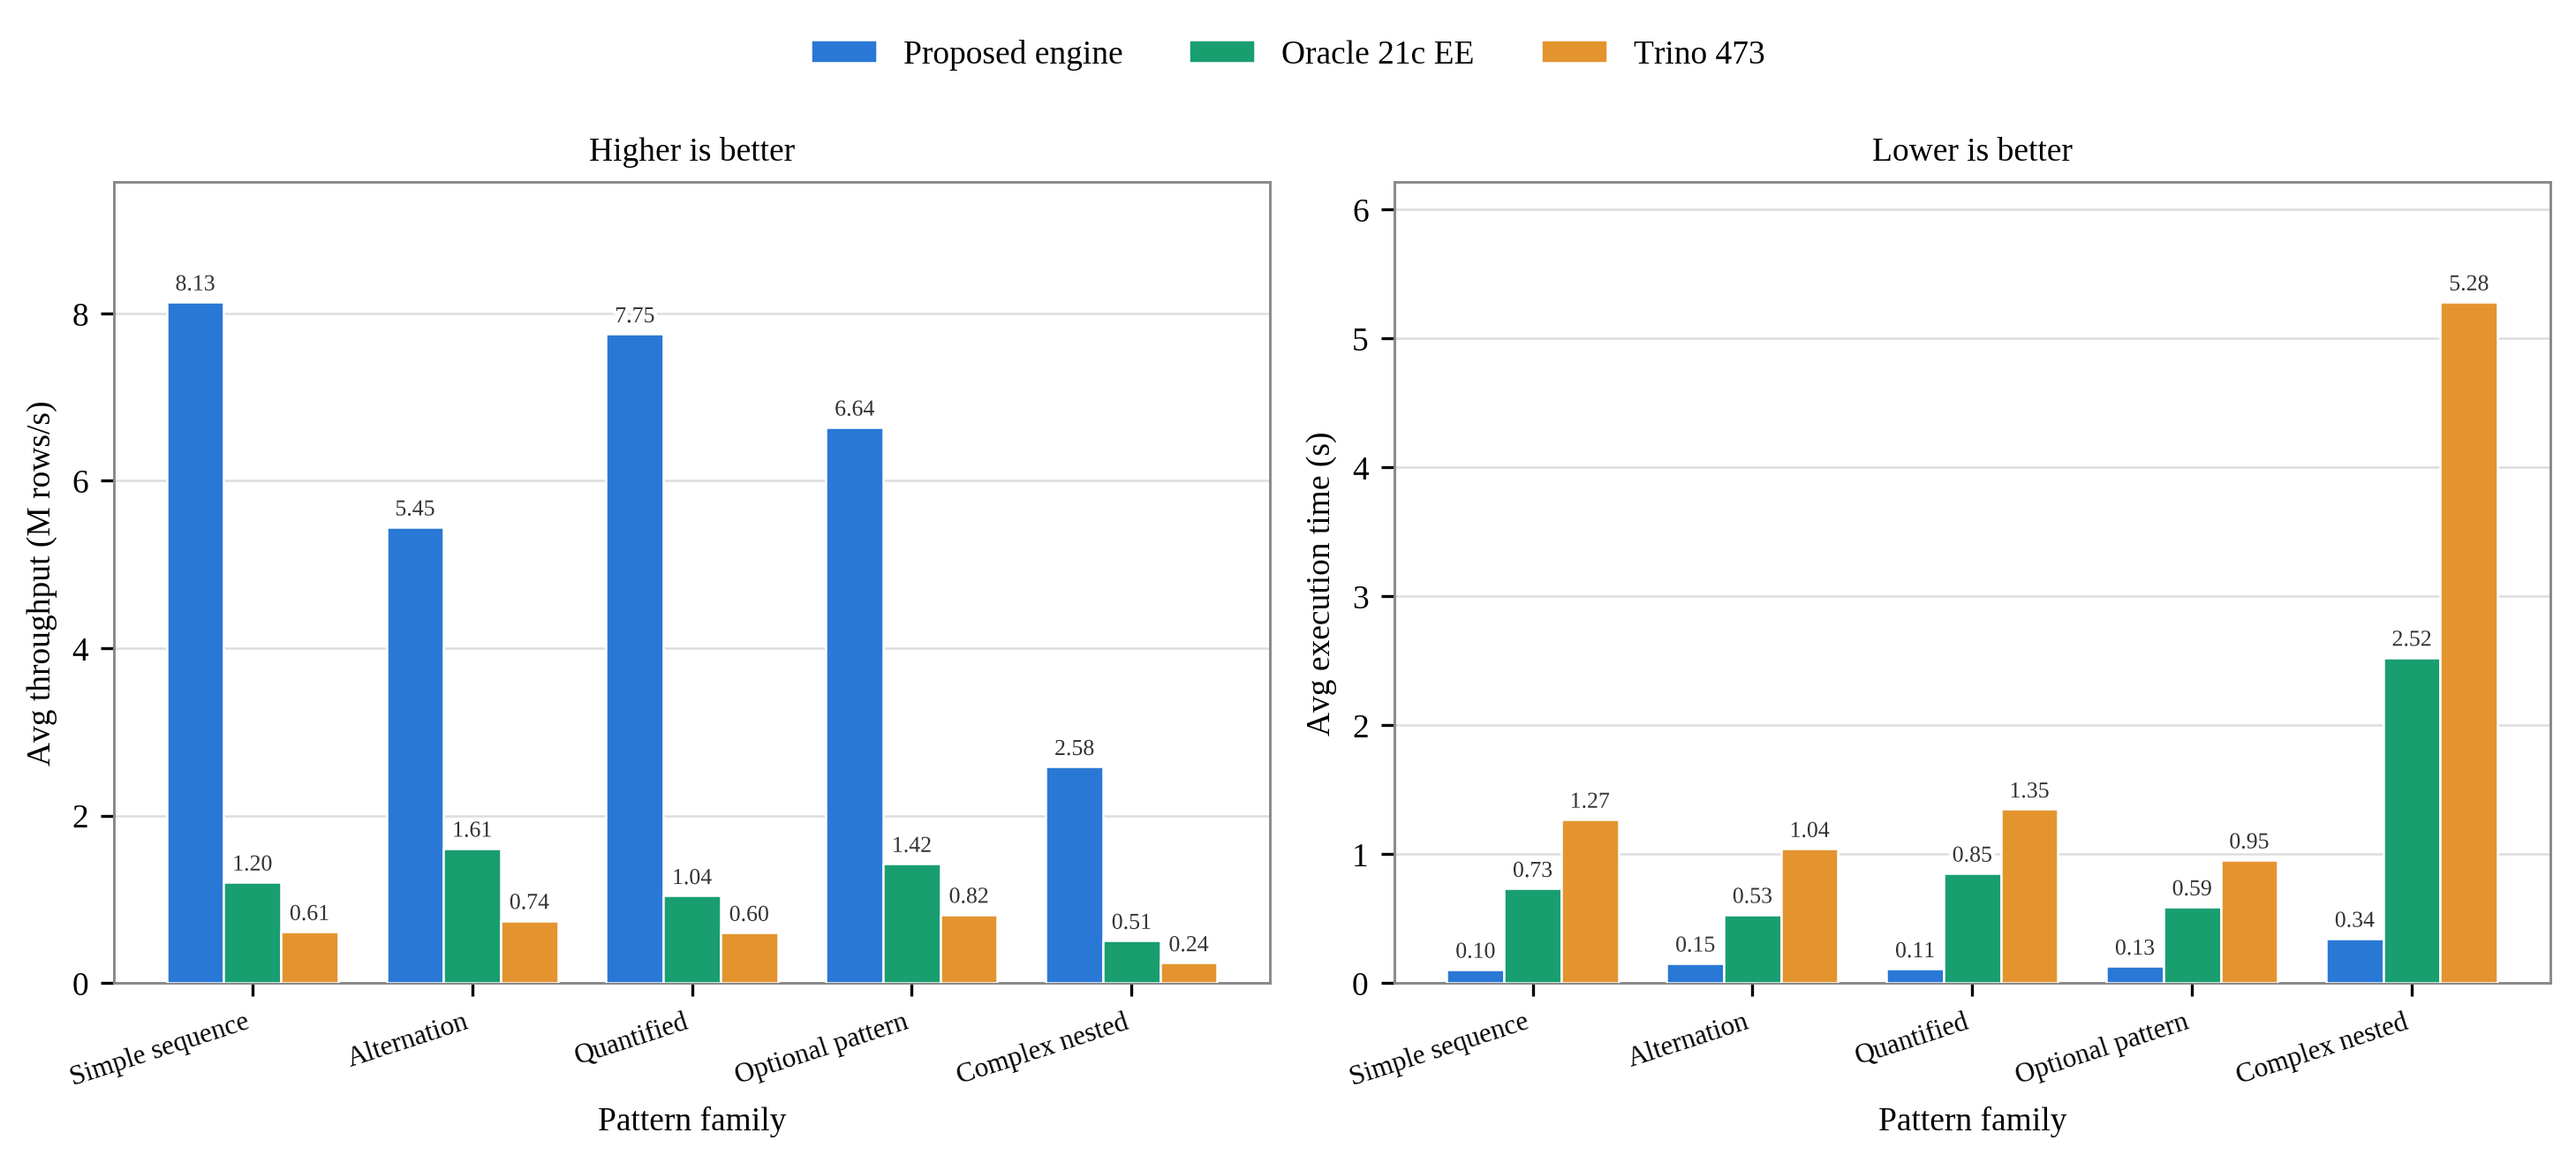
\includegraphics[width=\textwidth]{images/viz_summary_by_pattern.png}
  \caption[Performance summary by pattern]{Performance summary by
    pattern family.}
  \label{fig:summary_by_pattern}
\end{figure}

In Figure~\ref{fig:summary_by_pattern} each family is averaged over the
six sizes: throughput on the left (higher is better), time on the right
(lower is better).  The engine leads both measures on all five families.
The widest gap is \texttt{complex\_nested}, where Trino averages
5.28\,s against the engine's 0.34\,s, a factor of $15.4$.  The values are in
Table~\ref{tab:pattern_summary}.

\begin{figure}[htbp]
  \centering
  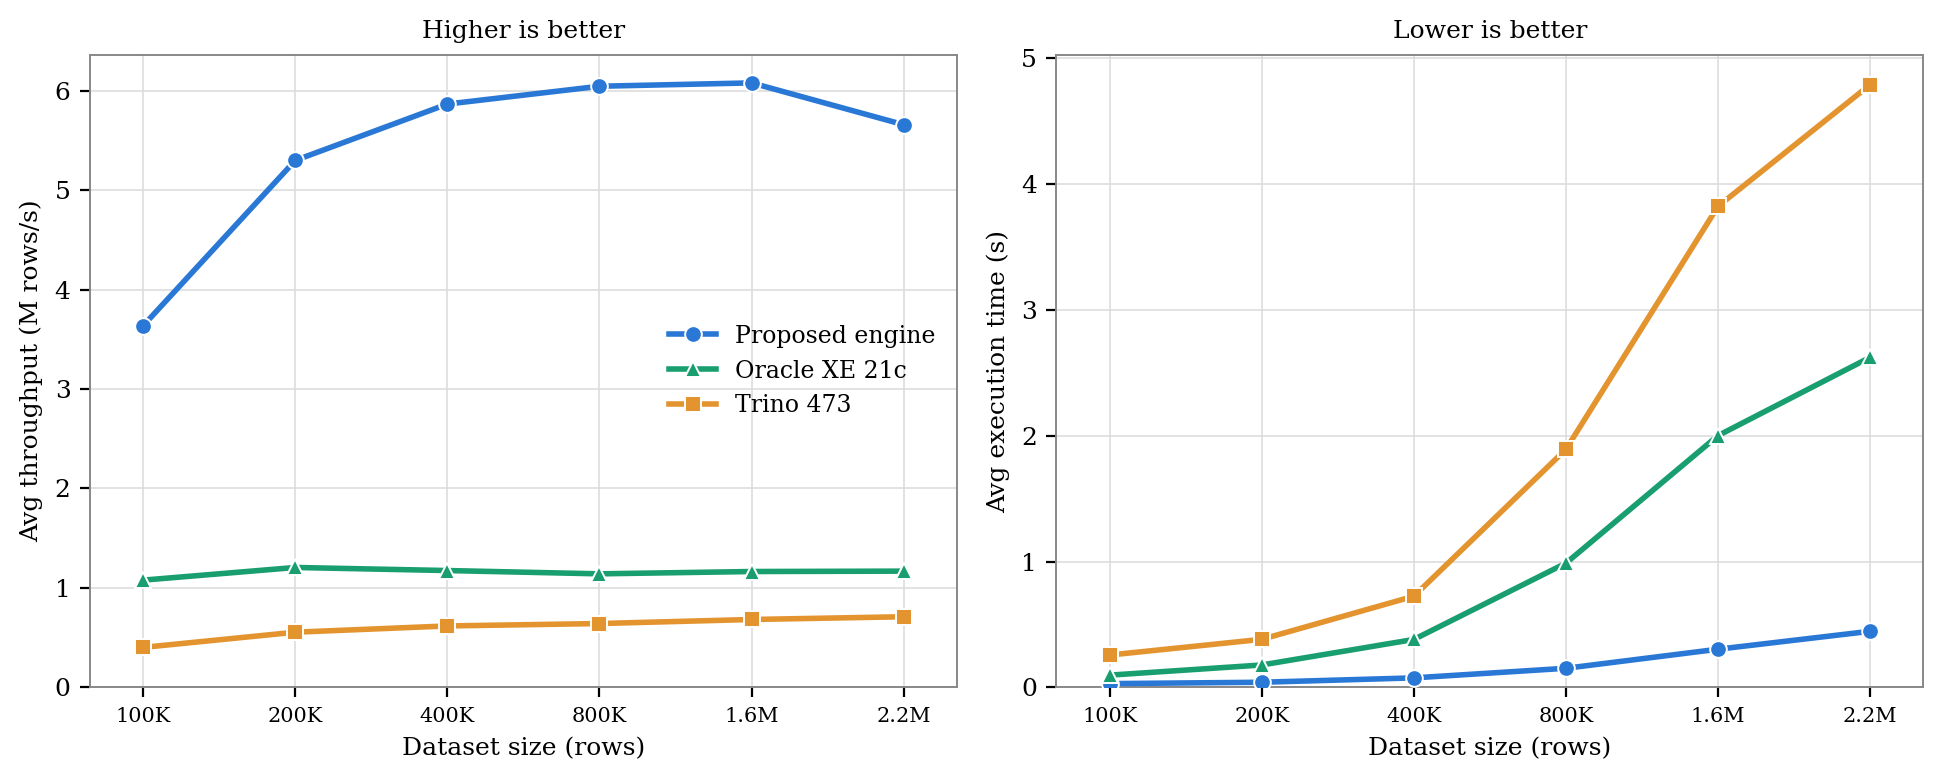
\includegraphics[width=\textwidth]{images/viz_summary_by_size.png}
  \caption[Performance summary by dataset size]{Performance summary by
    dataset size.}
  \label{fig:summary_by_size}
\end{figure}

Figure~\ref{fig:summary_by_size} groups the same data by size.  The
engine is fastest at every size, holding 5.0--6.9\,M rows/s as input
grows.  Per size it is about $9.3$--$13.3\times$ faster than
Trino and $4.3$--$7.0\times$ faster than Oracle.  The values are in
Table~\ref{tab:size_summary}.

\begin{figure}[htbp]
  \centering
  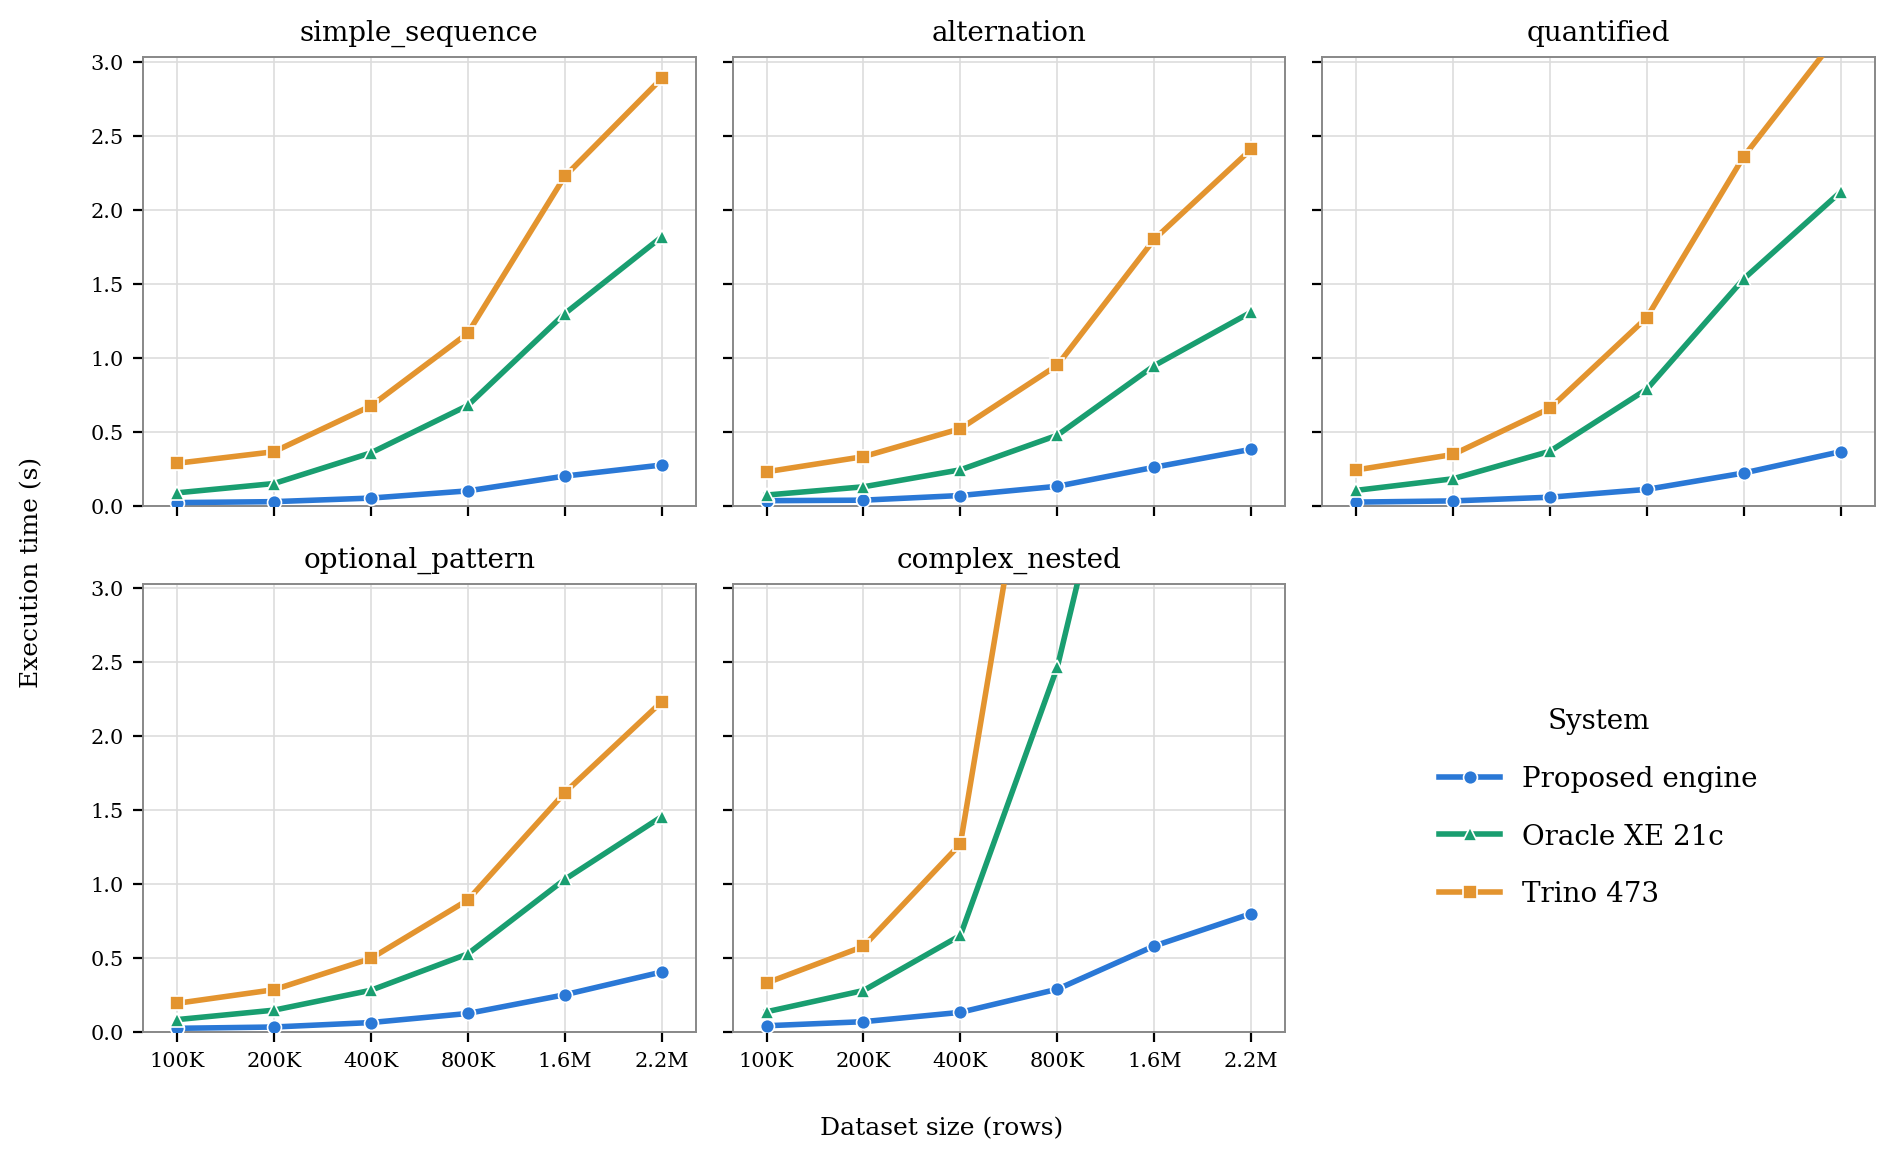
\includegraphics[width=\textwidth]{images/execution_times.png}
  \caption[Execution time by pattern, size, and system]{Execution time by pattern, size, and system.}
  \label{fig:execution_times}
\end{figure}

Figure~\ref{fig:execution_times} gives one time-versus-size panel per
pattern.  The engine (blue) is the lowest curve everywhere.  The margin widens most on
\texttt{complex\_nested}, where the databases bend upward past 400\,K
rows while the engine stays near-linear
(Table~\ref{tab:execution_times}).

% ................................................................
\subsection{Throughput by Pattern, Size, and System}
\label{subsec:eval-throughput}
% ................................................................

\begin{figure}[htbp]
  \centering
  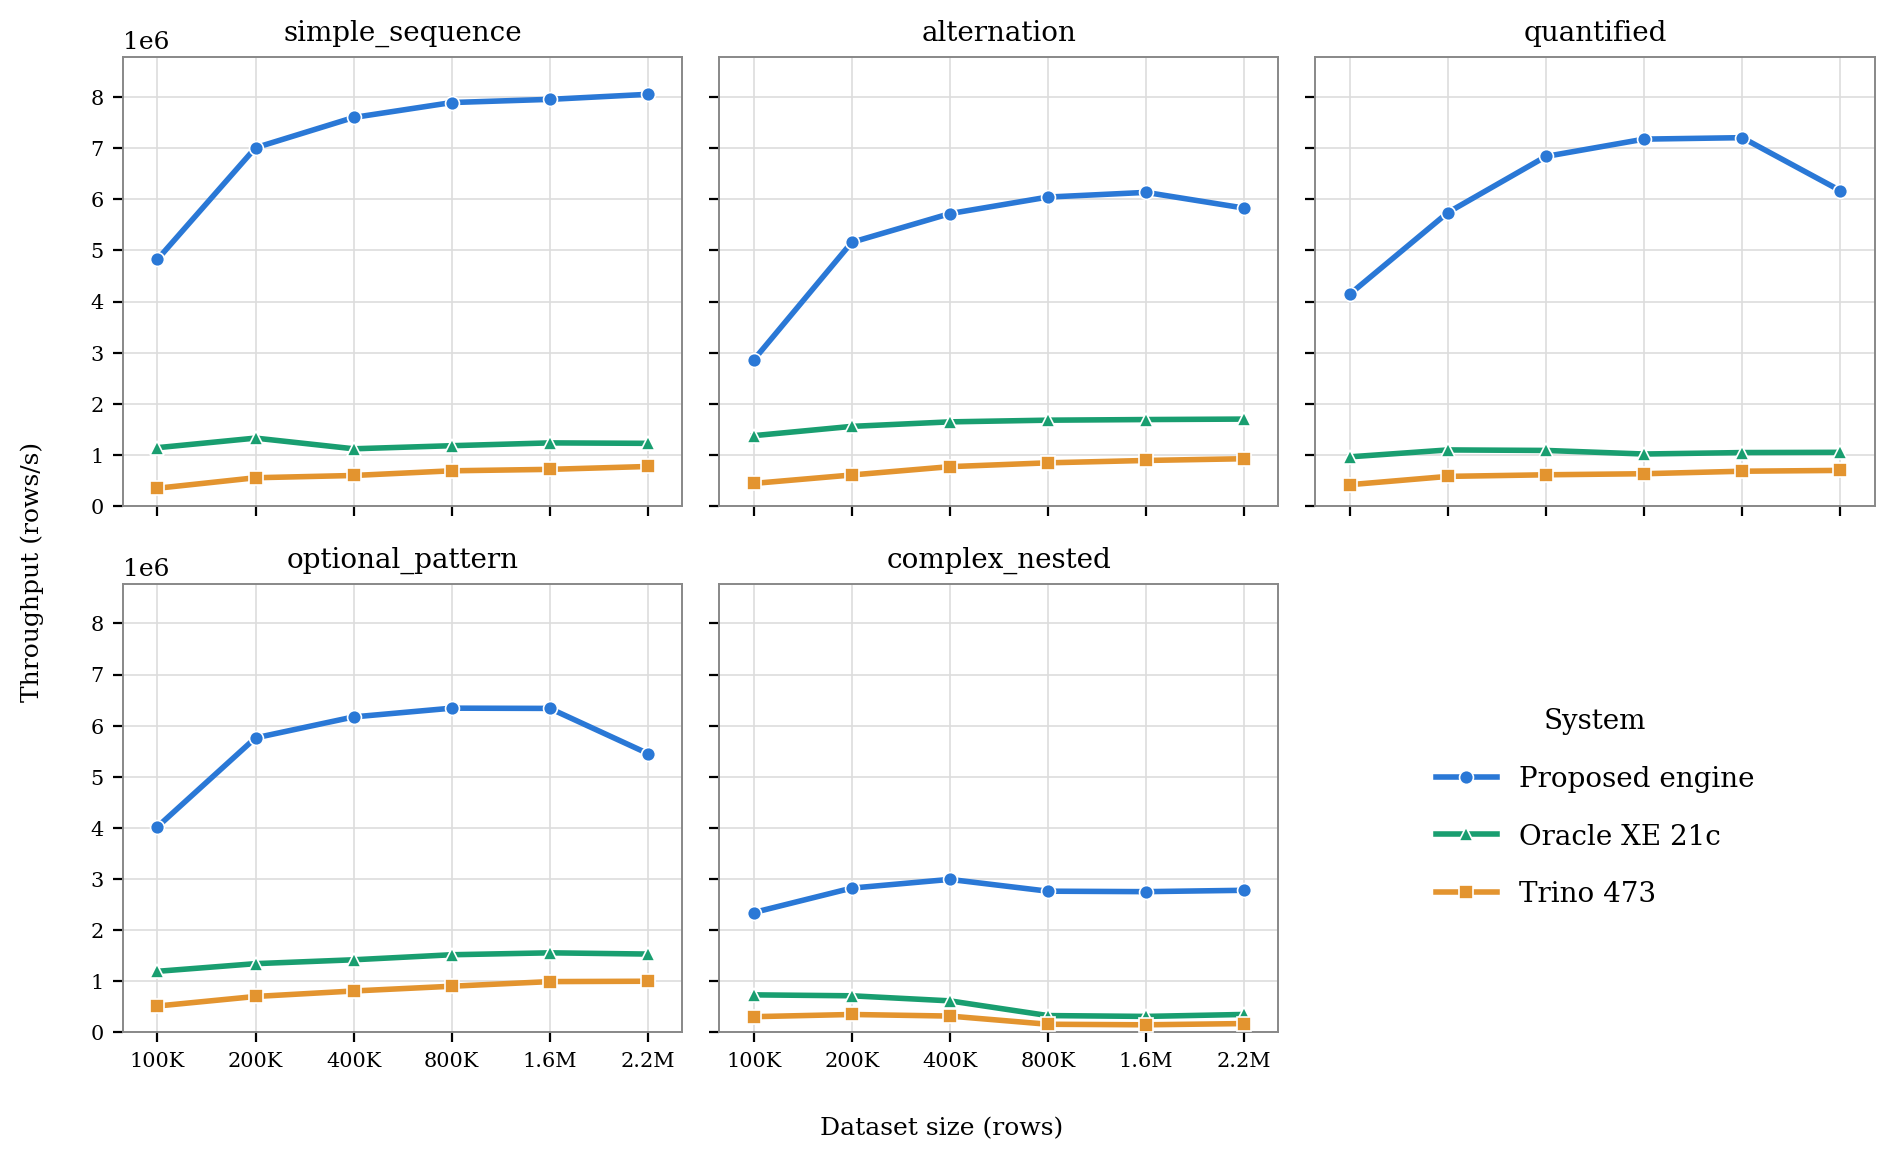
\includegraphics[width=\textwidth]{images/viz_throughput.png}
  \caption[Throughput by pattern, size, and system]{Throughput by pattern, size, and system.}
  \label{fig:throughput}
\end{figure}

Figure~\ref{fig:throughput} plots throughput, one panel per pattern;
higher is better.  Throughput is computed for each measured run, as
dataset size divided by that run's time, then filtered by the same
$1.5\times$ IQR rule and averaged.  The engine is the highest curve in
every panel
(Table~\ref{tab:throughput}).

% ................................................................
\subsection{Memory Metrics by Pattern, Size, and System}
\label{subsec:eval-memory}
% ................................................................

\begingroup\emergencystretch=3em
For the main benchmark, both memory metrics use the same cgroup~v2
\texttt{memory.current} counter.  It measures the dedicated engine
control group or the complete Trino or Oracle container every 50\,ms.
The boundaries are therefore operational rather than identical: the
engine value covers its Python process, while each database value
covers its server container and excludes the external client.  Shorter
allocation spikes can also fall between samples.\par\endgroup

The scripts divide byte counters by $1024^2$ and $1024^3$.  For compact
labels, MB and GB in the memory results therefore mean the binary units
MiB and GiB.

Each measured run has a five-second idle window.  Its average defines
the \emph{baseline}.  The \emph{absolute peak} is the largest query-time
sample, and the \emph{incremental peak} is that sample minus the
baseline.  The subtraction removes most fixed resident memory, such as
the already-loaded DataFrame, Oracle System Global Area (SGA), and
Trino JVM heap.  It does
not turn the values into an exact algorithm-only measurement.  As with
time, each reported memory value is the IQR-filtered mean over twenty
measured runs.

\emph{Query memory} (Figure~\ref{fig:query_memory};
Table~\ref{tab:memory_cache} in Appendix~\ref{app:benchmark-tables})
reports the incremental peak.  \emph{Footprint memory}
(Figure~\ref{fig:footprint_memory}; Table~\ref{tab:memory_footprint})
reports the absolute peak.  The footprint documents the practical
deployment cost of the resident engine or container, and is \emph{not} a
per-query or algorithm-level metric.

Two supporting values are recorded per cell in the benchmark evidence.
The first is a \emph{memory-per-million-rows} normalization: the
incremental peak divided by the input size in millions, meaningful
mainly at the larger sizes.  The second is each database's own per-query
counter, Trino's \texttt{peakMemoryBytes} and the high-water delta of
Oracle's session Program Global Area (PGA), which serve as cross-checks
below.

\begin{figure}[htbp]
  \centering
  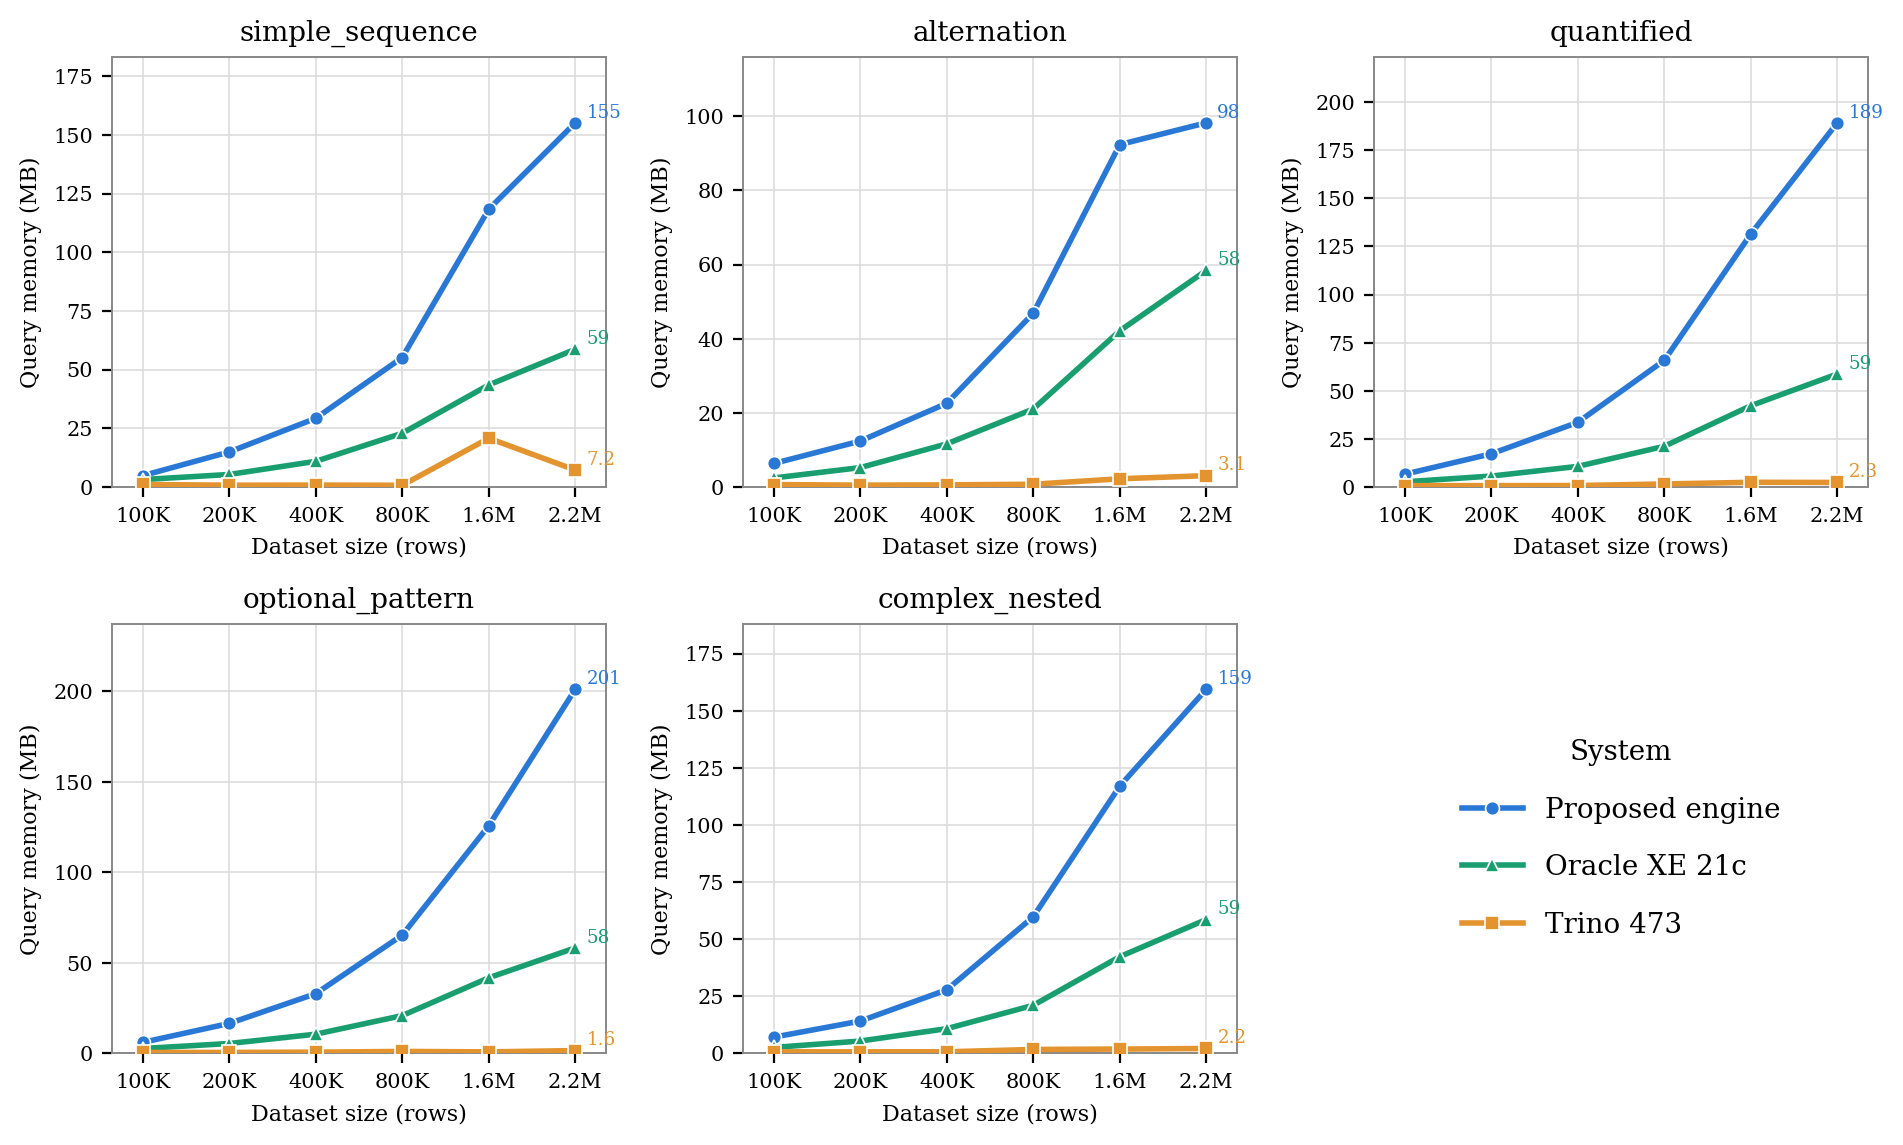
\includegraphics[width=\textwidth]{images/viz_query_memory.png}
  \caption[Query memory by pattern, size, and system]{Query memory (incremental peak) by pattern, size, and system.}
  \label{fig:query_memory}
\end{figure}

The engine's and Oracle's peaks rise roughly with size: the engine
5.9\,MB to 189\,MB, and Oracle 2.4\,MB to 58.7\,MB.  The engine's
incremental peak is the largest of the three (mean 64.5\,MB versus
Oracle's 23.6\,MB, about $2.7\times$).  This is consistent with the
compiled path creating whole-column masks and intermediate arrays.

One caveat for Trino is that the incremental cgroup measure observes
growth above an already-resident JVM heap.  It stays below 2.5\,MB in
27 of the 30 cells, with a largest value of 20.8\,MB.  Trino's native
\texttt{peakMemoryBytes} counter ranges from 1.3 to 41.5\,MB.  The two
counters have different scopes, so neither should be substituted for
the common footprint comparison.

\begin{figure}[htbp]
  \centering
  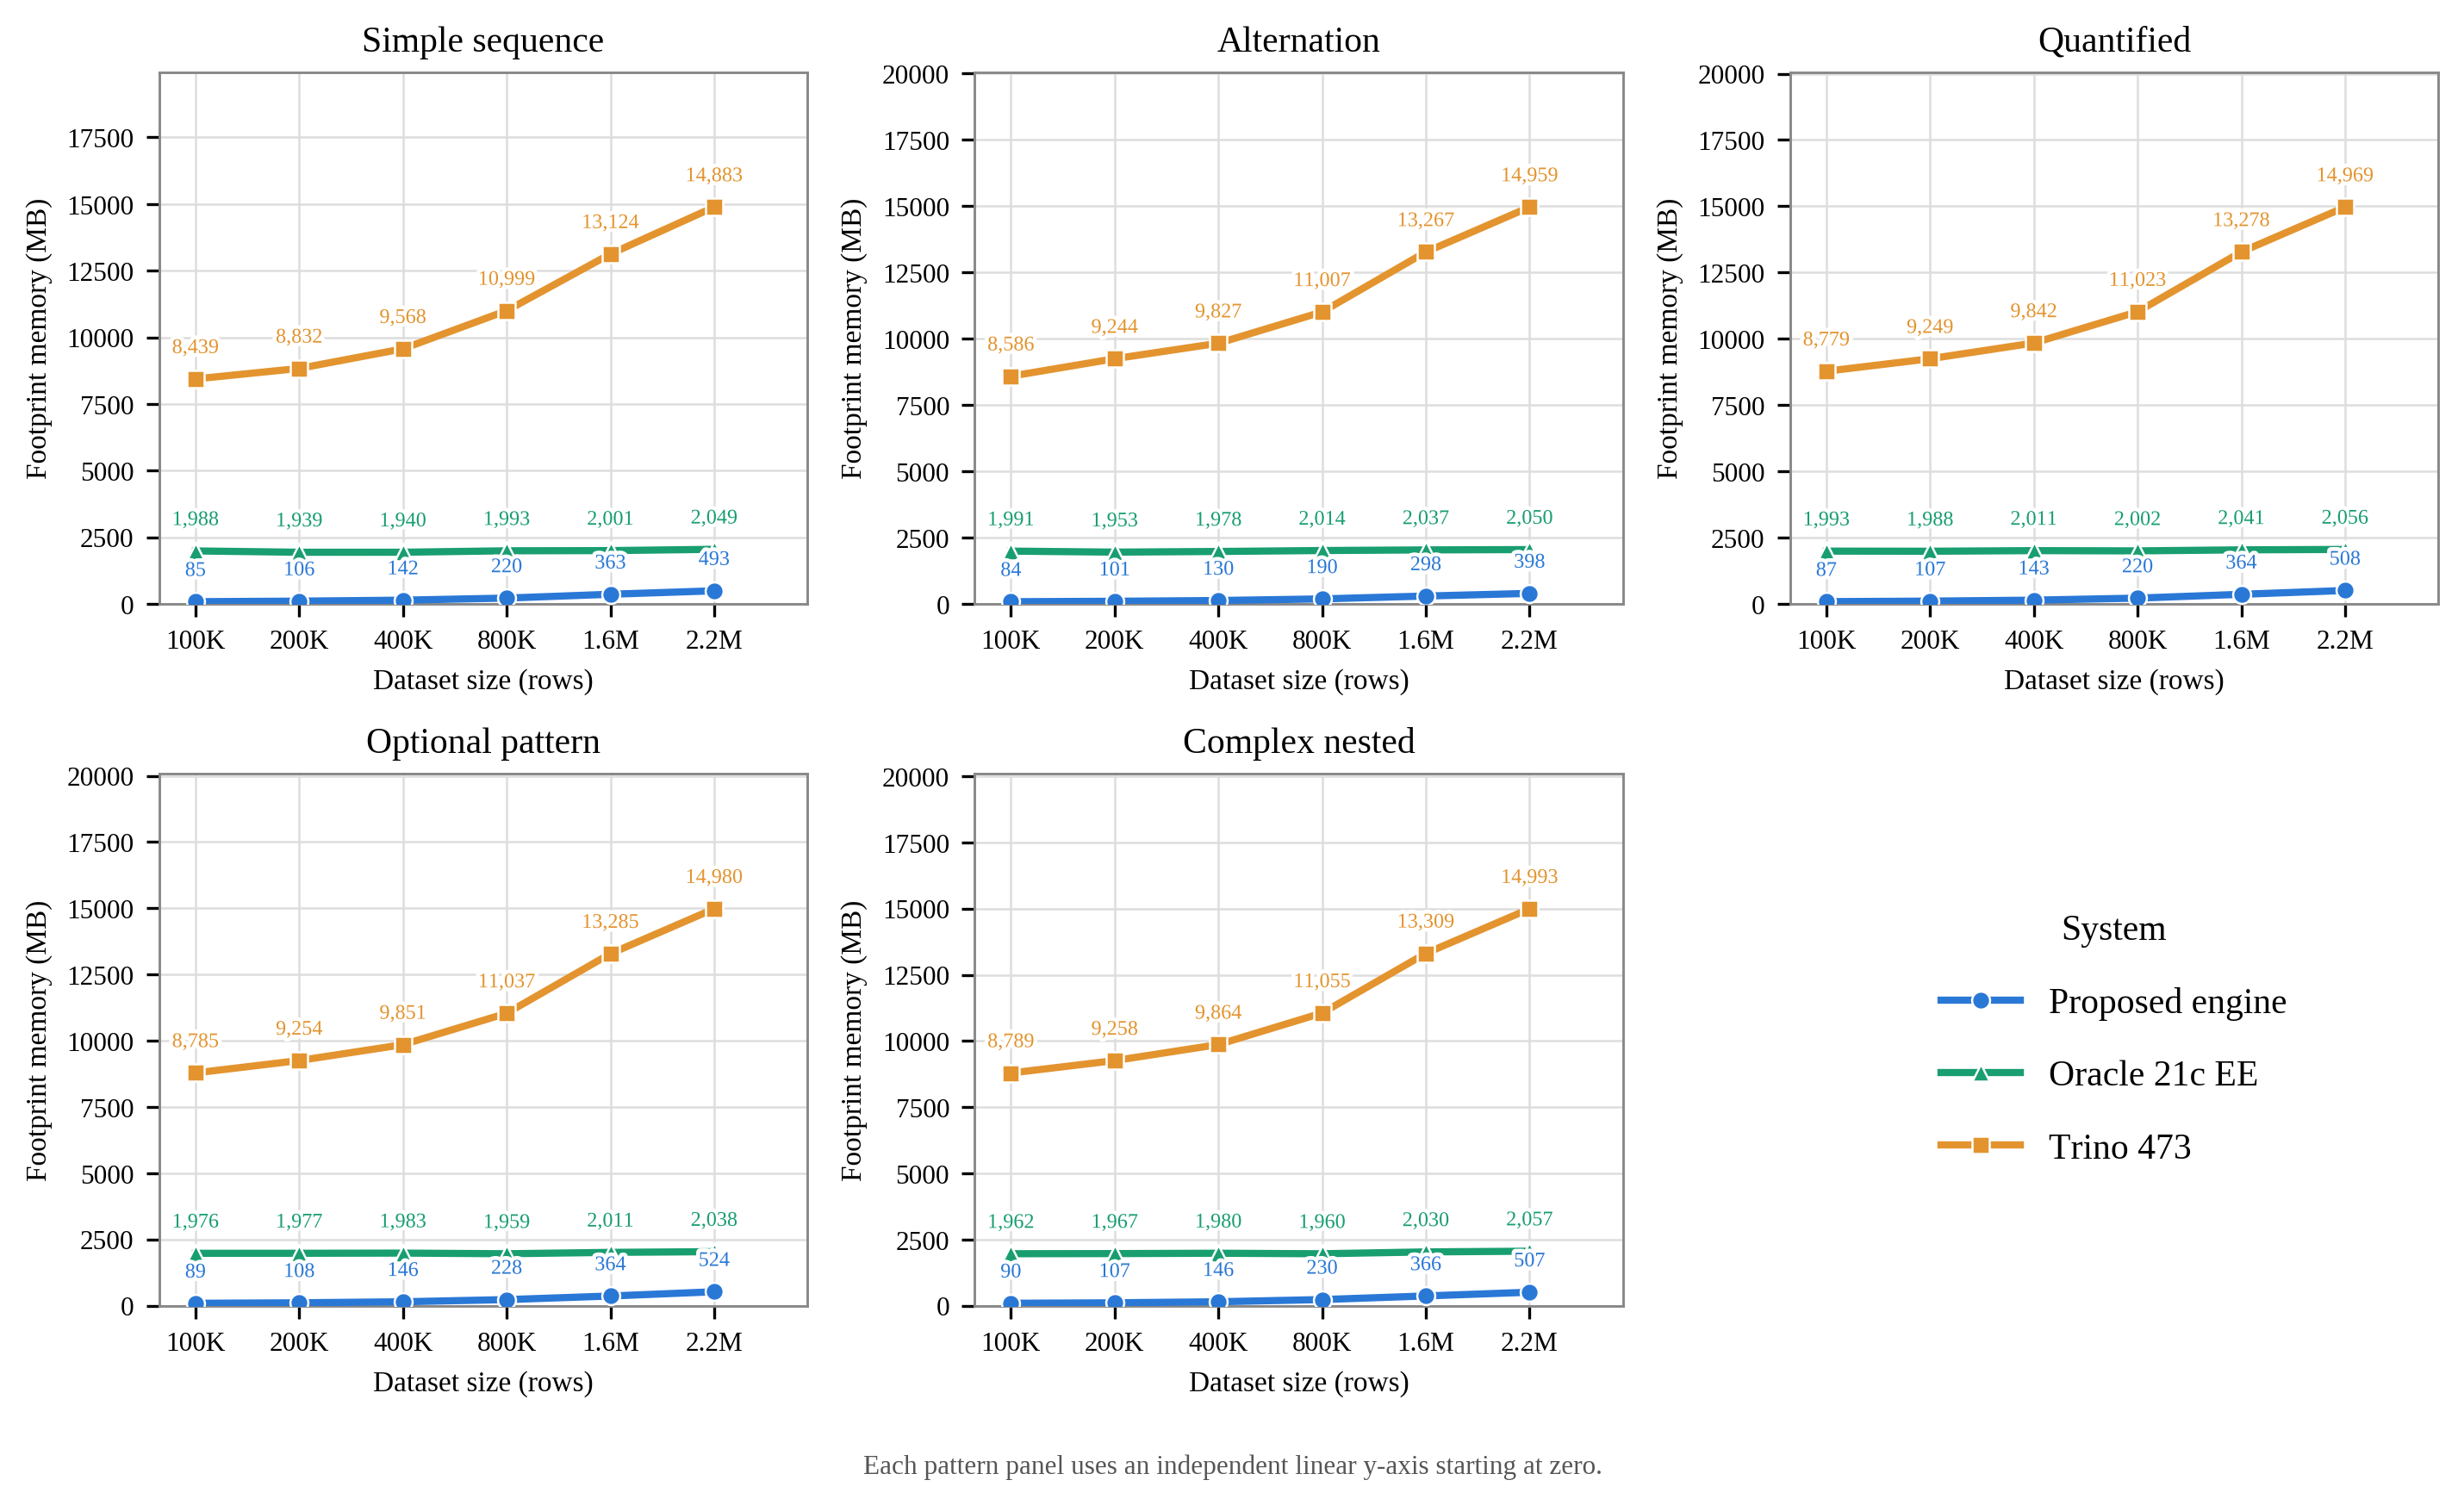
\includegraphics[width=\textwidth]{images/viz_footprint_memory.png}
  \caption[Footprint memory by pattern, size, and system]{Footprint memory (absolute peak) by pattern, size, and system.}
  \label{fig:footprint_memory}
\end{figure}

These deployment footprints have different boundaries.  The engine is
one Python process and peaks at 0.51\,GB.  The database values cover
whole containers: Trino uses 8.2--14.6\,GB because the table resides in
its JVM heap, while Oracle stays near 2.0\,GB.  Per-size restarts make
the measurements independent across sizes.  They show deployment cost;
per-query comparisons use Table~\ref{tab:memory_cache}.

% ................................................................
\subsection{Cross-System Summary}
\label{subsec:eval-key-findings}
% ................................................................

\begin{figure}[htbp]
  \centering
  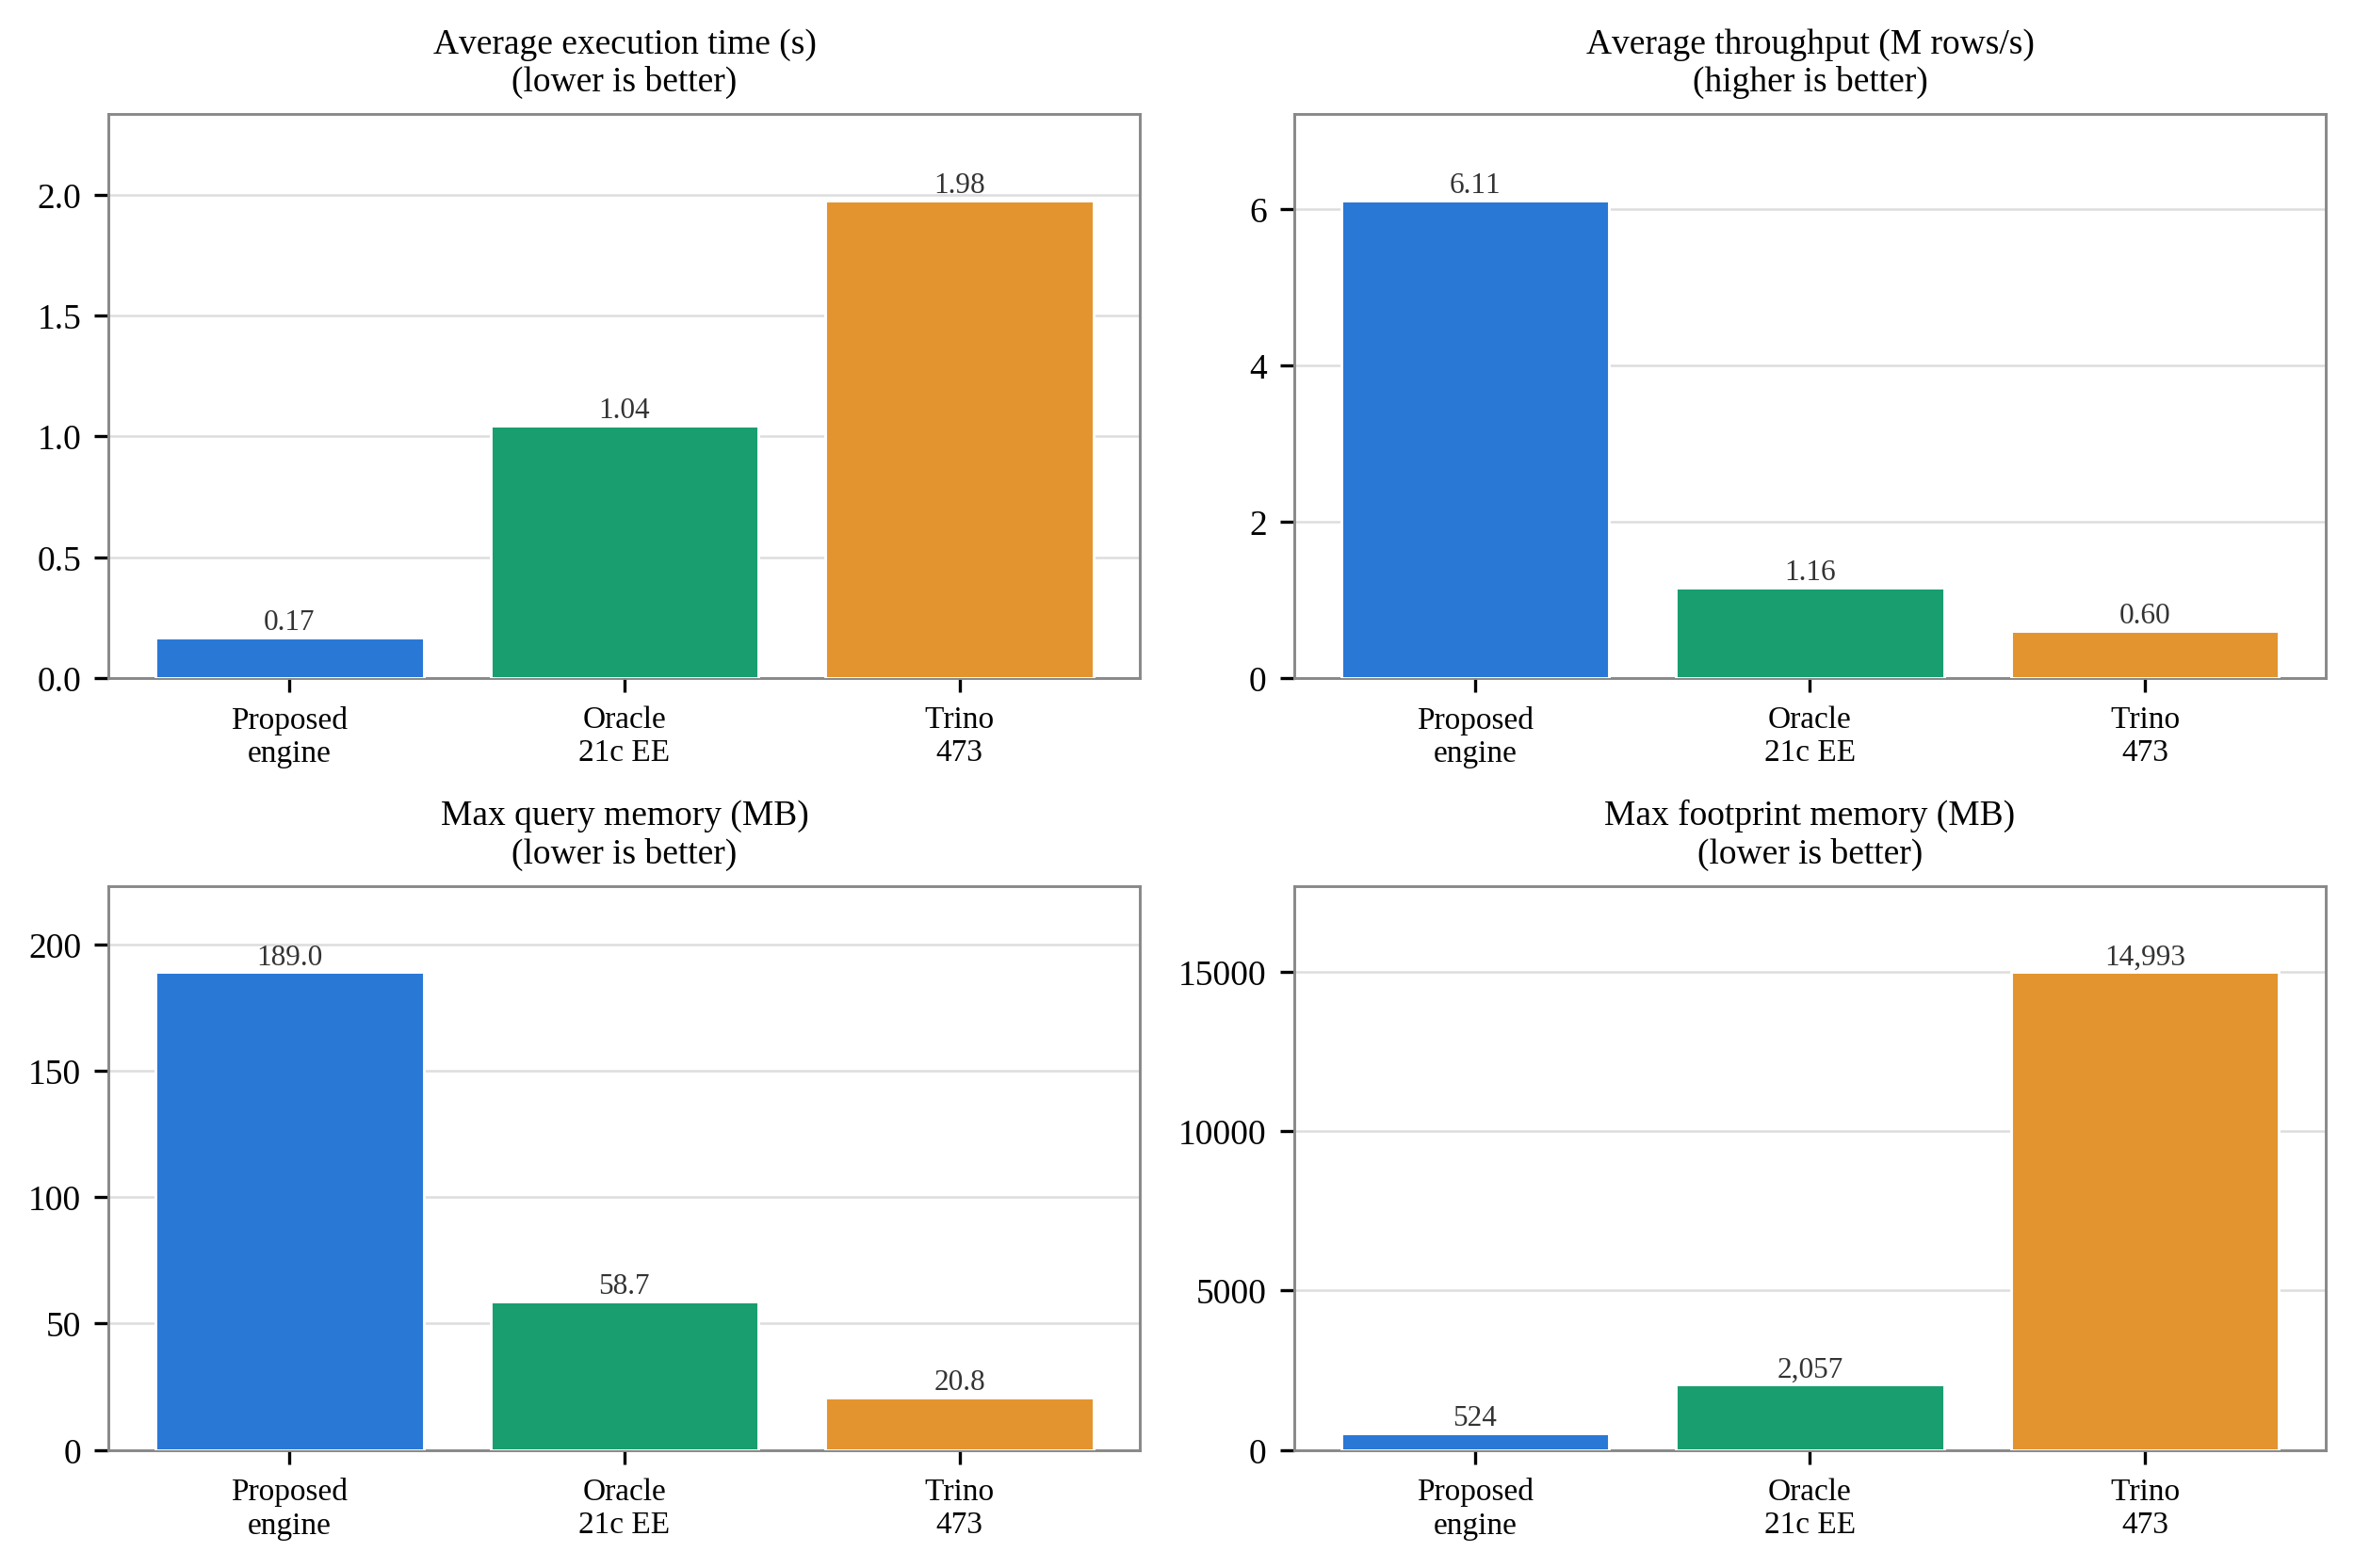
\includegraphics[width=0.95\textwidth]{images/viz_overall_stats.png}
  \caption[Overall benchmark statistics by system]{Overall benchmark
    statistics by system.}
  \label{fig:overall_stats}
\end{figure}

Figure~\ref{fig:overall_stats} has four panels, each with one bar per
system.  \emph{Average execution time} is the mean of the 30 cell
means: 0.17\,s for the engine, against 1.04\,s for Oracle and
1.98\,s for Trino.  The engine runs inside the process that already
holds the data, so it avoids the planning, storage, and
client-transfer layers the databases still pay for.  It also compiles
supported conditions to column operations.  \emph{Average throughput}
is the same 30 cells read as rates: 6.11\,M\,rows/s, against 1.16 and
0.60.  The rate does not fall as data grows, which is what near-linear
time means, and the spread from 2.49 to 9.40\,M\,rows/s tracks pattern
structure rather than size.

\emph{Max query memory} is the largest rise above the idle baseline.
The engine is highest at 189\,MB.  The compiled path is vectorized: it
builds whole-column masks and intermediate arrays over all input rows
instead of walking row by row.  The cost therefore follows the input,
not the result.  It stays between 56 and 90 bytes per input row in all
30 cells, and the 189\,MB cell returns 95{,}650 rows while a
186\,MB cell returns 276{,}776.  This is the memory side of the design
that gives the speed.  Trino's 20.8\,MB is growth above an
already-resident heap, not a like-for-like figure.
\emph{Max footprint memory} is the largest total the process or
container reached.  Here the order reverses: 524\,MB for the engine,
2{,}057\,MB for Oracle, and 14{,}993\,MB for Trino.  The boundaries
differ: one Python process against a complete database container, and
Trino is the largest because the table is held in its JVM heap.  It is
a deployment cost, not a per-query one.  The
engine leads on time, throughput, and total footprint, and trades that
for the highest per-query memory (Table~\ref{tab:overall_stats}).

\begin{figure}[htbp]
  \centering
  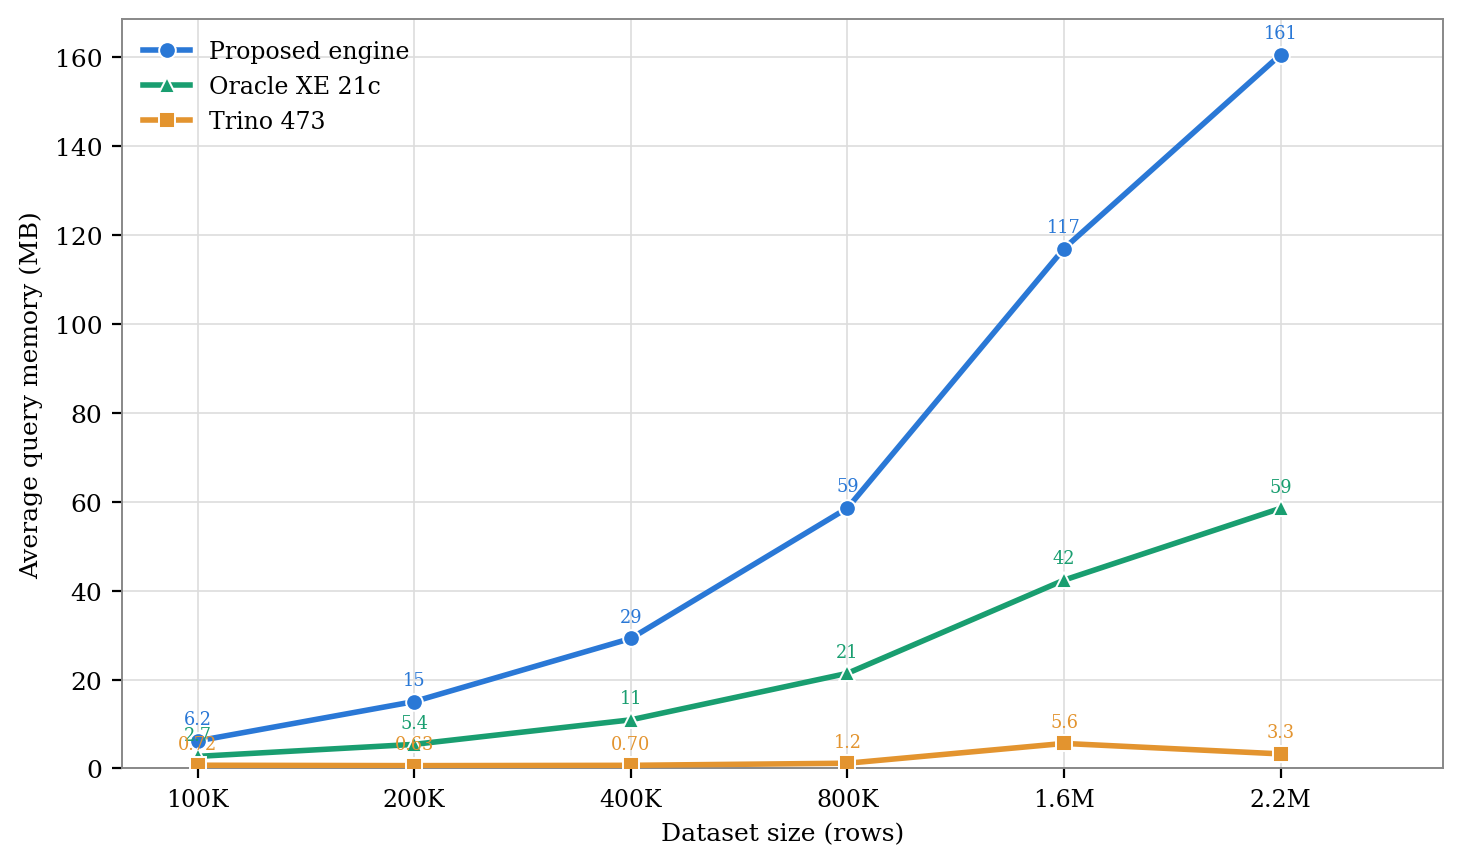
\includegraphics[width=0.82\textwidth]{images/viz_avg_memory_by_size.png}
  \caption[Average query memory by dataset size]{Average query memory
    by dataset size.}
  \label{fig:avg_memory_by_size}
\end{figure}

Averaged over the five patterns (Figure~\ref{fig:avg_memory_by_size}),
the engine's per-query memory rises with size.  It stays the highest of
the three (Table~\ref{tab:avg_memory_by_size}).

\begin{figure}[htbp]
  \centering
  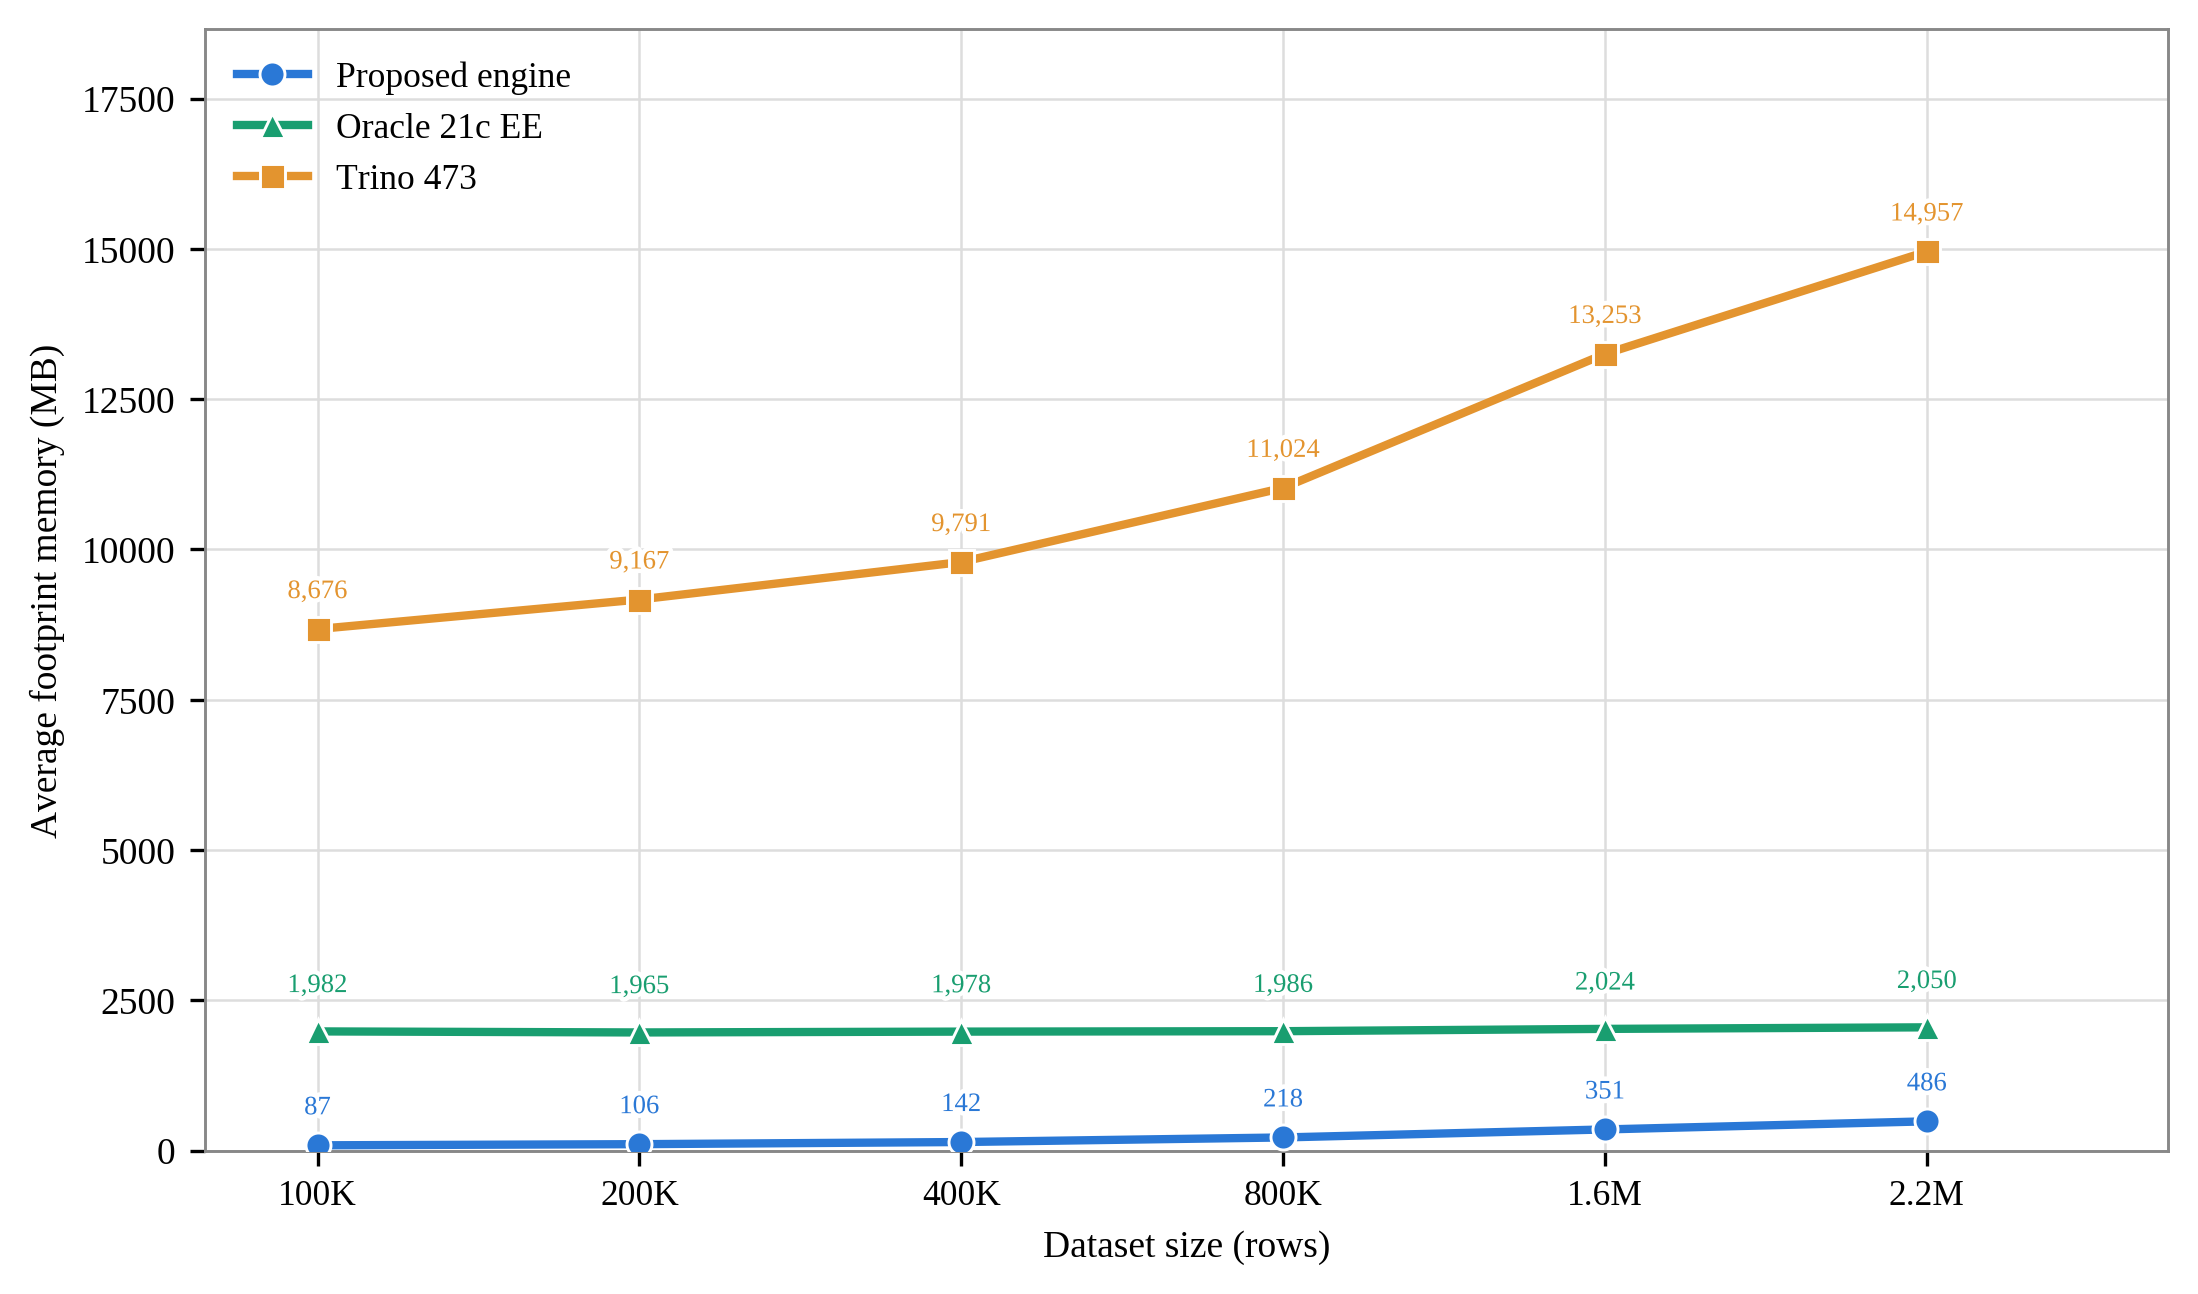
\includegraphics[width=0.82\textwidth]{images/viz_avg_footprint_by_size.png}
  \caption[Average footprint memory by dataset size]{Average footprint
    memory by dataset size.}
  \label{fig:avg_footprint_by_size}
\end{figure}

The footprint picture inverts (Figure~\ref{fig:avg_footprint_by_size}).
The engine's single process stays well below the Trino and Oracle
containers at every size (Table~\ref{tab:avg_footprint_by_size}).

All 90 system cells completed, and all 30 pattern--size combinations
agreed across the three systems.  The engine had the lowest mean time
(0.17\,s, against 1.04\,s for Oracle and 1.98\,s for Trino).  It also
had the highest incremental query peak but the lowest total footprint.
Run-to-run variation remained low after warmup and IQR filtering.  The
detailed values are reported once in
Appendix~\ref{app:benchmark-tables}.  These results describe the
selected workload and resource configuration; they do not establish
universal superiority.

Figure~\ref{fig:relative_comparison} puts the two databases against the
engine, drawn as a $1\times$ reference.

\begin{figure}[htbp]
  \centering
  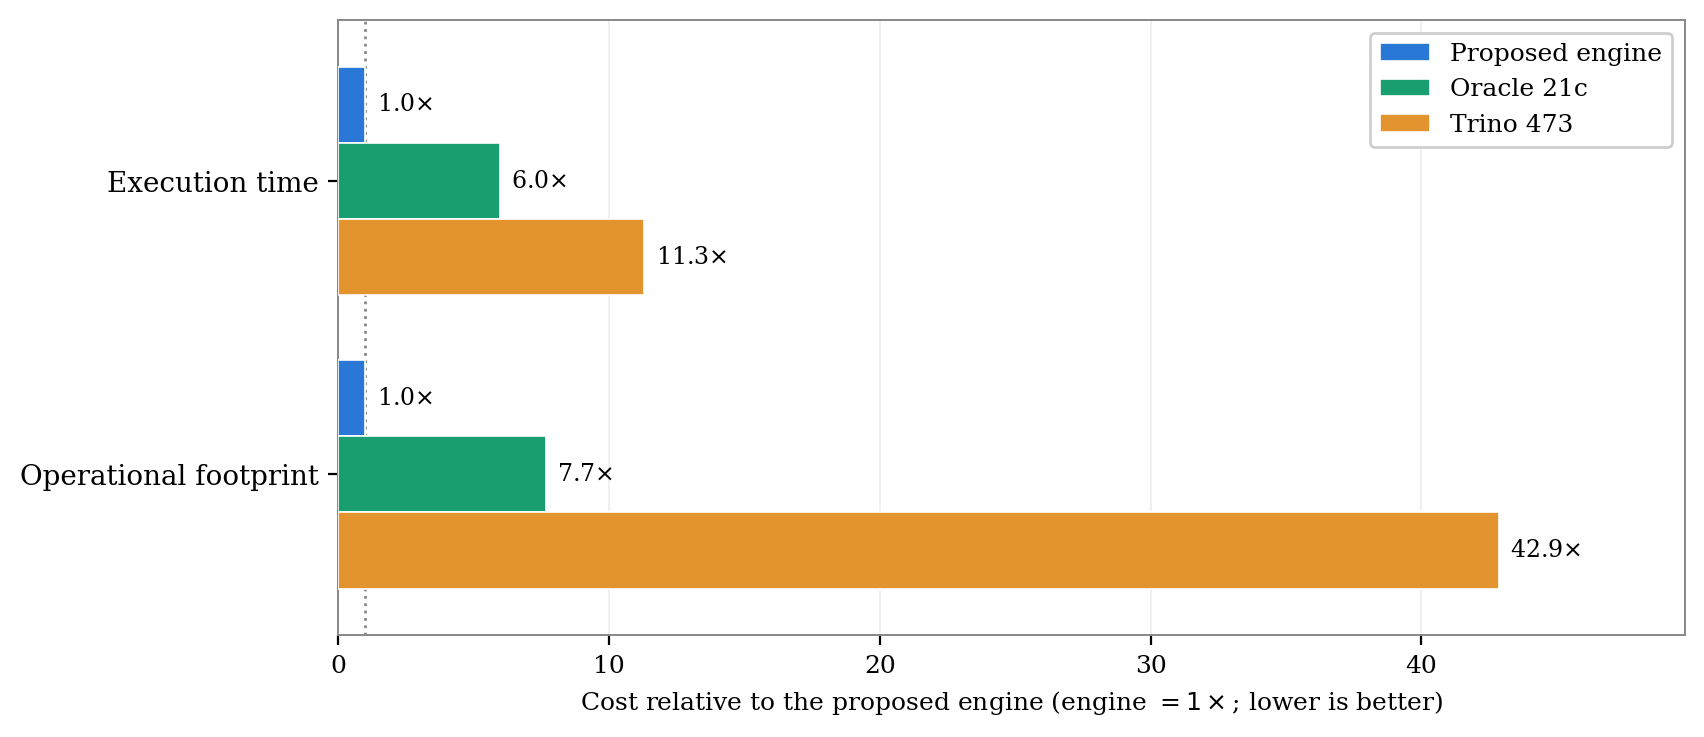
\includegraphics[width=0.95\textwidth]{images/viz_relative_comparison.png}
  \caption[Proposed engine relative to each SQL engine]{Cost of each
    database relative to the proposed engine (engine $=1\times$).}
  \label{fig:relative_comparison}
\end{figure}

Each bar is a database's average time or footprint as a multiple of the
engine's (blue $1\times$ line; lower is better).  Oracle needs
$6.2\times$ the time and $8.6\times$ the footprint; Trino $11.8\times$
and $48.1\times$.  Throughput mirrors the time result.  The engine's
one trade-off is higher incremental query memory, because the compiled
path creates whole-column working arrays (about $2.7\times$ Oracle's
mean incremental peak).  It is shown in
Figure~\ref{fig:query_memory}; signed percentages are in
Table~\ref{tab:relative_comparison}.

% ................................................................
\subsection{Sensitivity and Boundary Analysis}
\label{subsec:eval-ordering}
\label{subsec:eval-worst-cases}
% ................................................................

The main matrix uses ordered input and row-local predicates.  Two
sensitivity cases remove these advantages: shuffled input and a
state-dependent predicate.  Both are measured across all three
systems.

\paragraph{Sensitivity case 1: shuffled input.}
The benchmark orders by an already-monotonic \texttt{seq\_id}, so the
engine's $O(n)$ check skips its sort.  The matrix was rerun with every
input deterministically shuffled, which makes the engine enter its
$O(n\log n)$ sorting branch.  The query still restores the same logical
order.  All 90 system cells completed, and all 30 pattern--size
combinations still agreed across systems.  Scenario~A is ordered and
Scenario~B is shuffled.  The difference measures sensitivity to
physical input order; it is not a direct profile of the sort operator
inside each database.

\begingroup\emergencystretch=3em
The proposed-engine values describe the benchmark revision recorded in
Appendix~\ref{app:provenance}.  The Oracle and Trino values were retained from the earlier
unordered campaign under the same one-core, 32\,GB, five-warmup,
twenty-run protocol.  As in the main benchmark, the systems ran
sequentially.  Figure~\ref{fig:ordering_scenarios} shows the result.\par\endgroup

\begin{figure}[htbp]
  \centering
  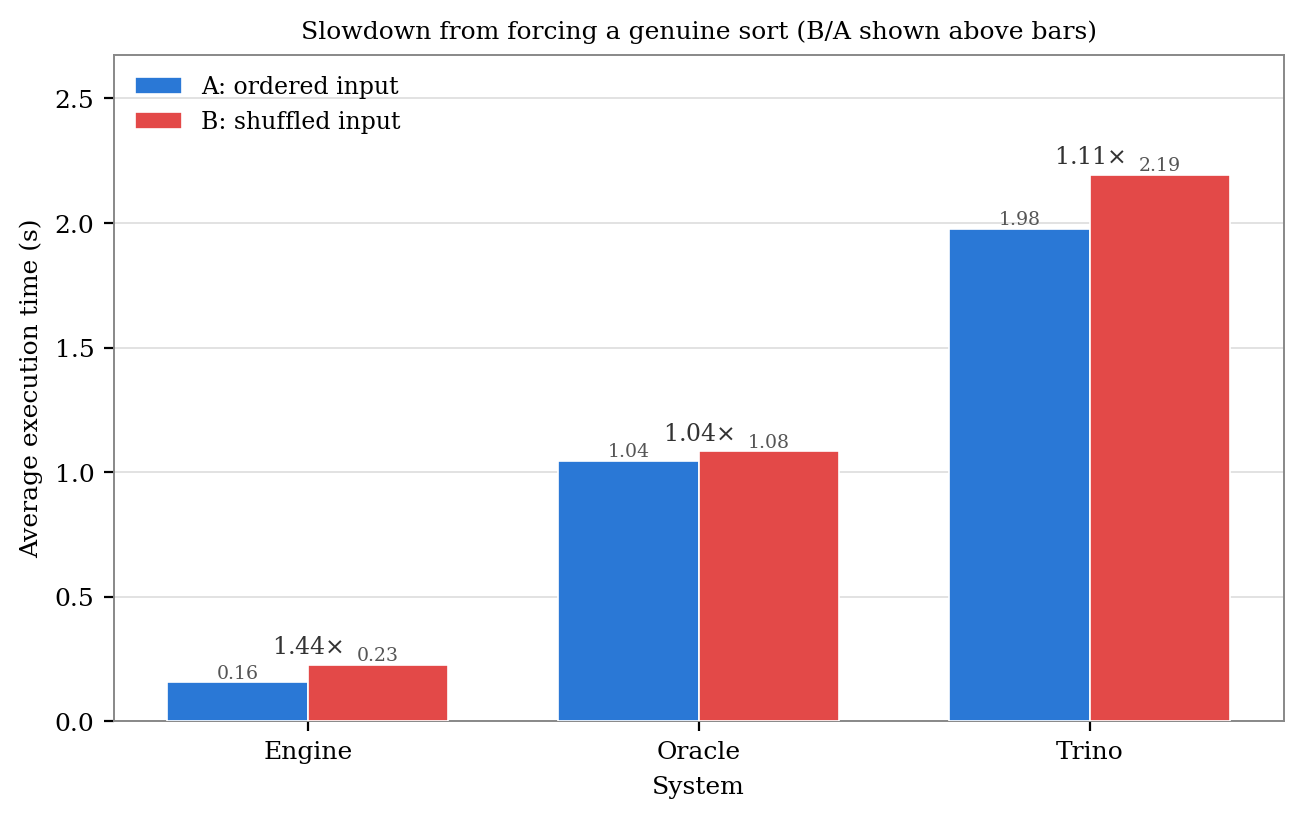
\includegraphics[width=0.78\textwidth]{images/viz_ordering_scenarios.png}
  \caption[Ordered vs shuffled input by system]{Average execution time
    on ordered vs shuffled input, by system.}
  \label{fig:ordering_scenarios}
\end{figure}

Each pair is a system's ordered (A) and shuffled (B) average; the
number above is the B/A slowdown.  Scenario~A is the main matrix and
Scenario~B repeats it with every input shuffled.  Each A/B comparison
uses the same logical rows and query, but the changed physical layout
can also affect caching and compression.  The engine shows the largest
slowdown ($1.43\times$):
$1.70\times$ for \texttt{simple\_sequence}, $1.69\times$ for
\texttt{quantified}, and $1.19\times$ for
\texttt{complex\_nested}.  Oracle and Trino change by
$1.04$--$1.11\times$.  Their internal plans were not profiled, so this
smaller change is reported without assuming that they used the same
sort plan in both scenarios.  Most important, the ranking holds: at
2.22\,M rows the engine is still
about $4.5\times$ faster than Oracle and $8.8\times$ than Trino under
shuffled input (against $6.2\times$ and $11.2\times$ ordered).  So the
advantage is not an artifact of the ordered shortcut: it survives when
the engine must sort
(Tables~\ref{tab:ordering_scenarios}--\ref{tab:ordering_by_size}).

\begin{figure}[htbp]
  \centering
  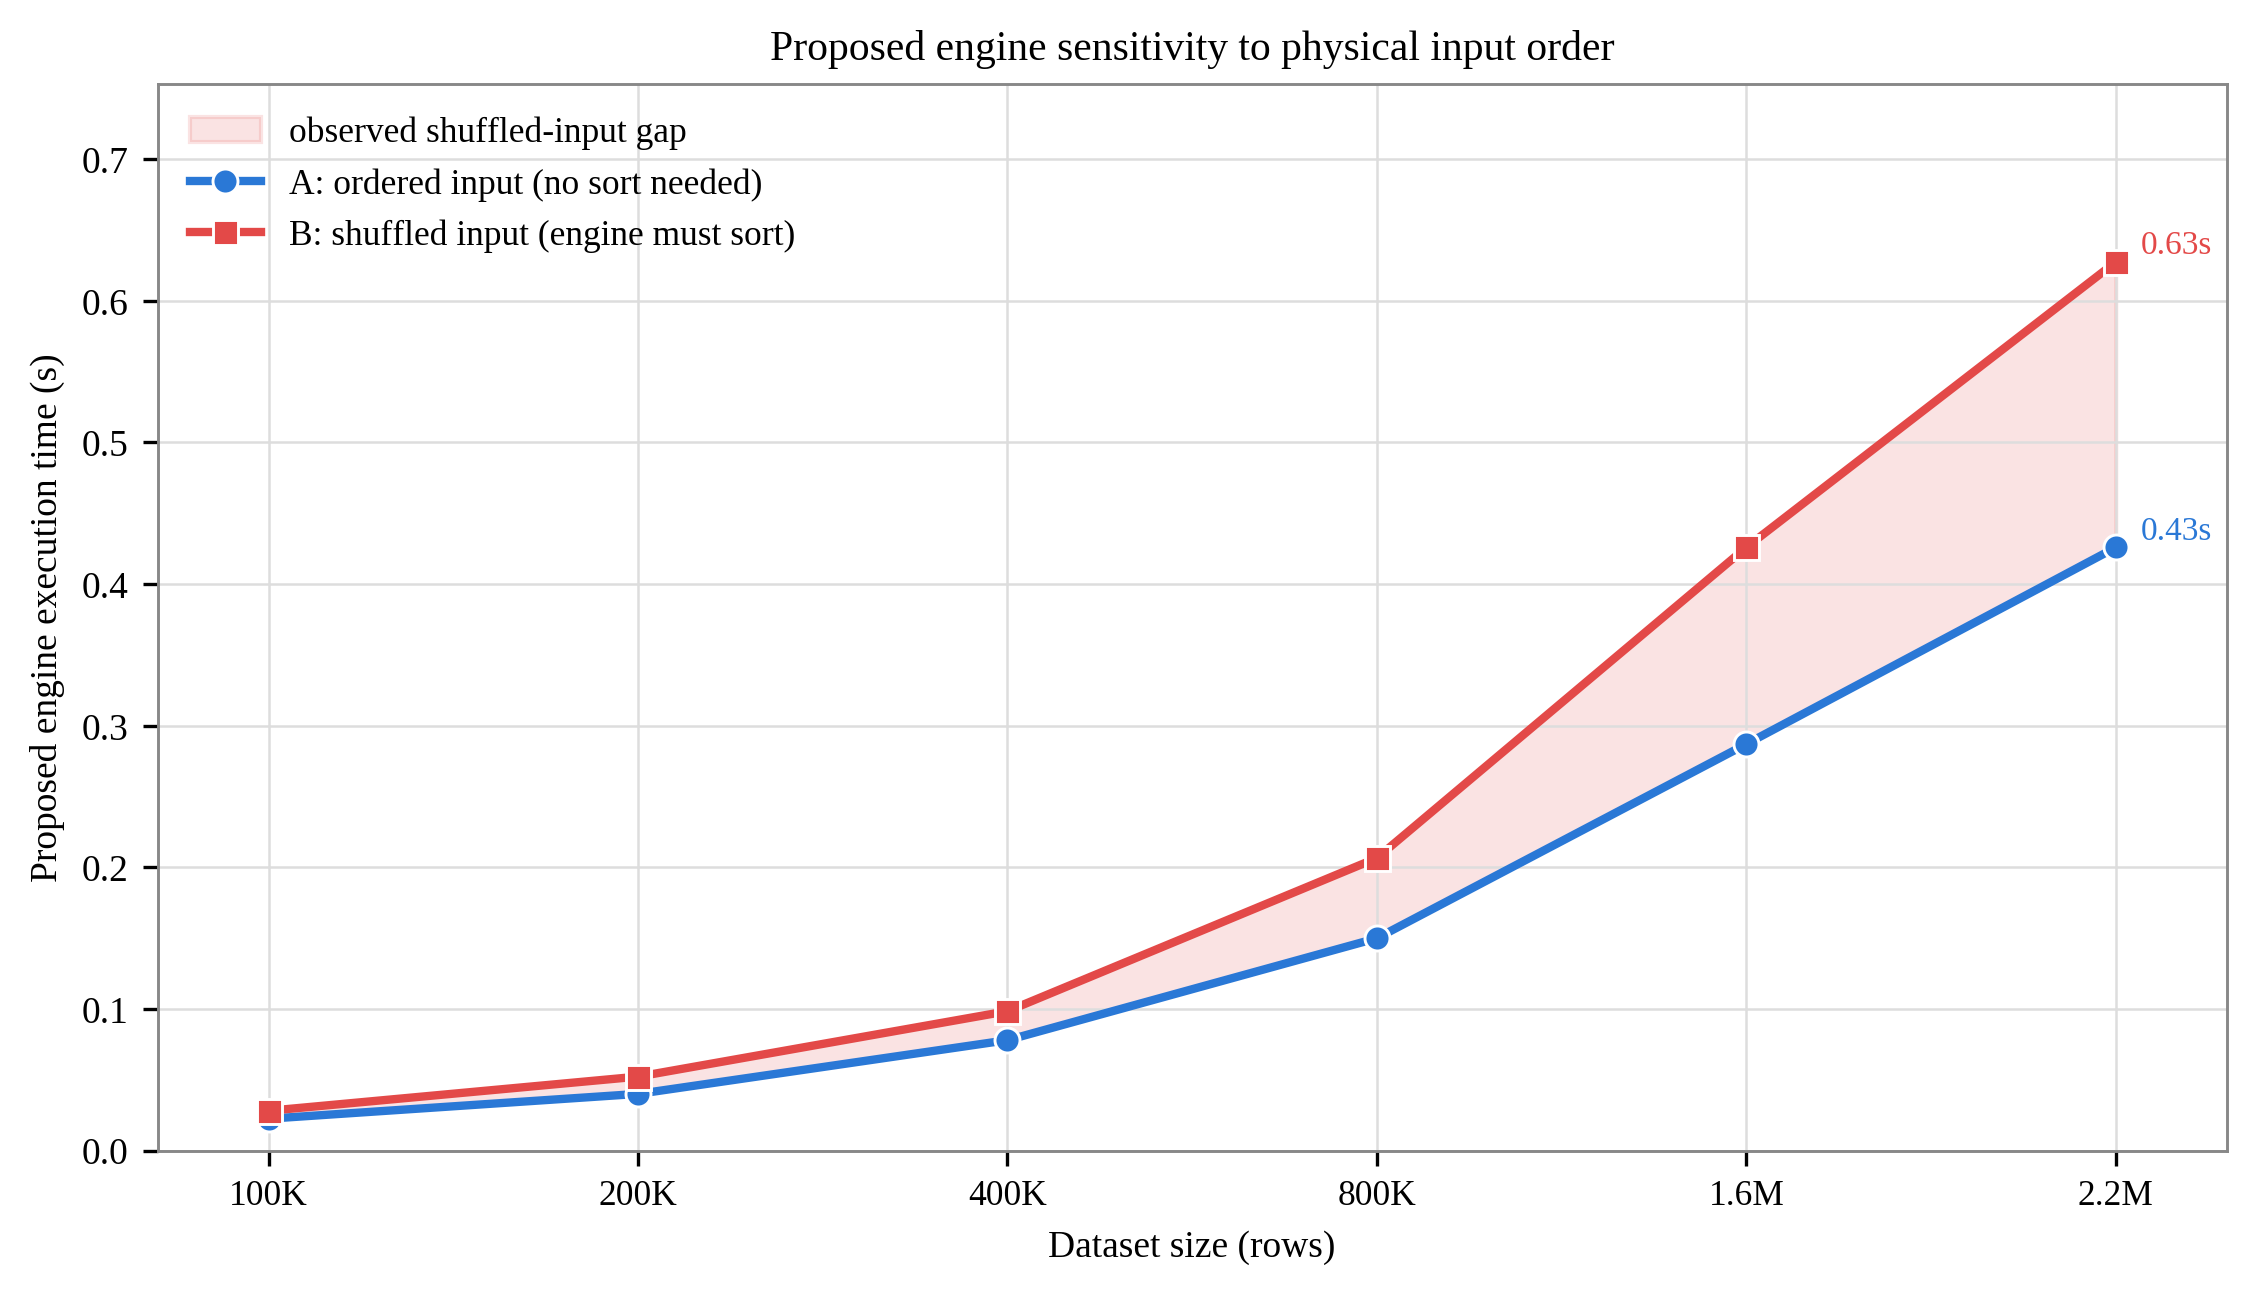
\includegraphics[width=\textwidth]{images/viz_sort_cost_scaling.png}
  \caption[Ordered and shuffled engine time]{Engine time on
    ordered vs shuffled input, across sizes.}
  \label{fig:sort_cost_scaling}
\end{figure}

Figure~\ref{fig:sort_cost_scaling} compares
the engine on ordered (no sort) and shuffled (forced sort) input.  Both
grow close to linearly over these six sizes, exactly what the reading
note of Section~\ref{subsec:eval-complexity} predicts, since the log
factor barely moves over this range.  The shaded gap is the extra
latency associated with shuffled input, including the engine's sort.
It is 0.20\,s at 2.22\,M rows (0.43\,s ordered versus 0.63\,s
shuffled), and its normalization by $n\log_2 n$ stays within the same
order of magnitude
(Table~\ref{tab:sort_cost_by_size}).  Over this measured range, the
shuffled-input penalty remains smaller than the total latency.

\paragraph{Sensitivity case 2: a state-dependent predicate.}
Shuffling changes ordering work but leaves the predicates row-local.
A state-dependent predicate cannot use the same row-local
Boolean matrix.  To show this boundary,
the \texttt{simple\_sequence} query's \texttt{DEFINE} becomes
\texttt{B AS category='B' AND price > AVG(A.price)}, a running
aggregate that depends on the match so far.  Trino and Oracle evaluate
it natively.  All three produce identical output, so the semantic
comparison is valid.

The repetition counts differ from the main matrix.  The recorded
engine values use five warmups and twenty measured runs per size.  The retained
Trino and Oracle values use one warmup and two measured runs per size.
The systems ran sequentially.  This test therefore shows the
performance boundary, but its database means have less repetition than
the main benchmark.  Figure~\ref{fig:worstcase_coverage} plots the
three systems on it.

\begin{figure}[htbp]
  \centering
  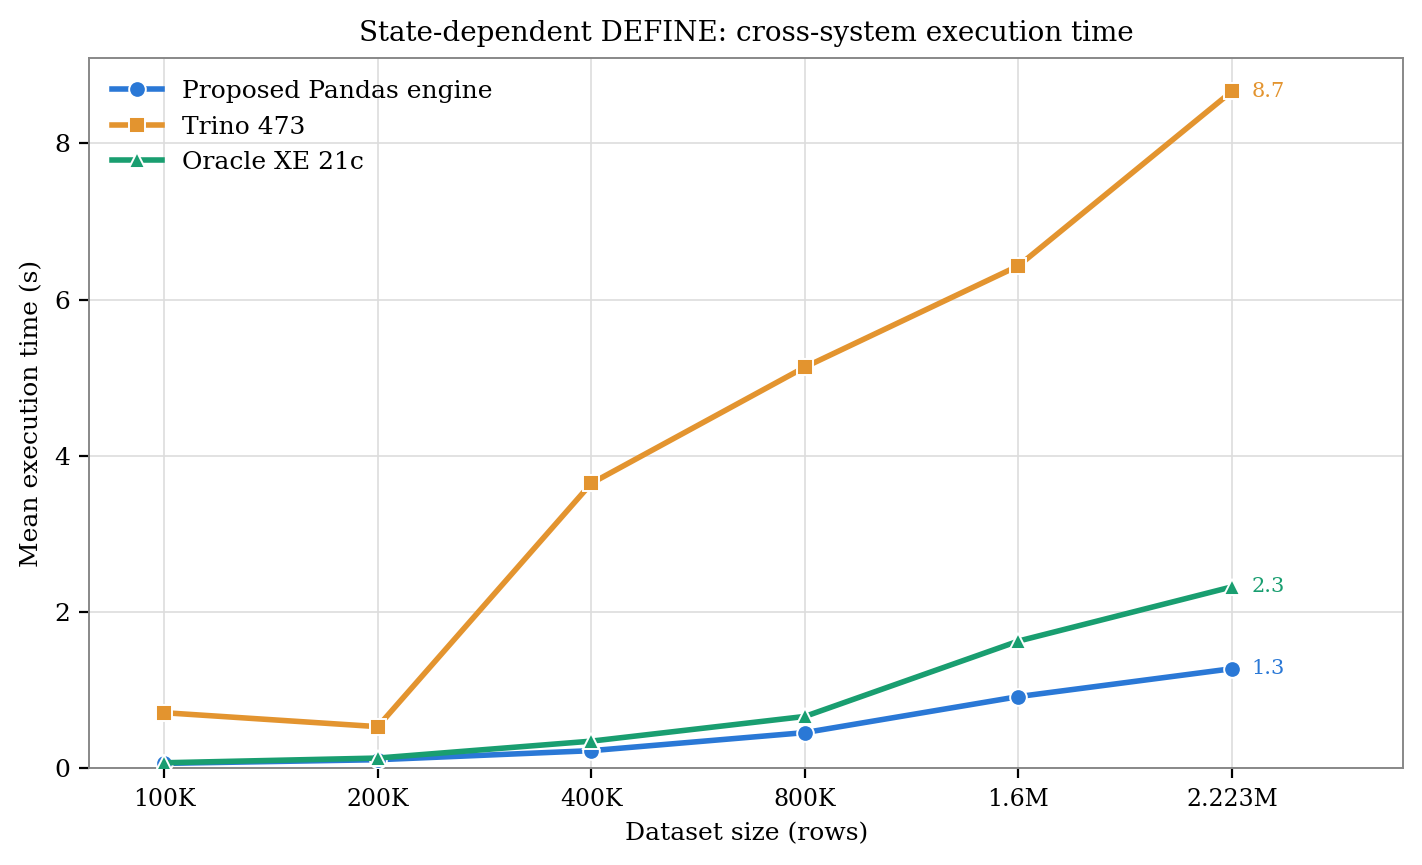
\includegraphics[width=0.78\textwidth]{images/viz_worstcase_xsys.png}
  \caption[Pattern-driven worst case, all systems]{Execution time on a
    state-dependent \texttt{DEFINE} query, all systems.}
  \label{fig:worstcase_coverage}
\end{figure}

An earlier recorded run reversed the ranking.  The engine was the
\emph{slowest} system at every size, 64.41\,s at 2.22\,M rows, because
the generic exact evaluator repeatedly recomputed
\texttt{AVG(A.price)} as the tentative match grew.  The exact matcher
now compiles this form into an incremental plan.  It updates the
\texttt{A} prefix state on append and rollback instead of recomputing
the aggregate.  This evaluated query is linear, but it is not a
row-local vectorized predicate.  It takes $1.28$\,s at 2.22\,M rows,
about $50\times$ faster than the earlier $64.41$\,s result, with identical output
($181{,}147$ matches).  The engine is now fastest here
too, $1.2$--$1.8\times$ ahead of Oracle and $5.0$--$15.9\times$ ahead
of Trino (Table~\ref{tab:worstcase_coverage}).

This is one compiled incremental form, not a general solution for all
state-dependent expressions.  Supported forms outside the compiled
plans still use the generic exact evaluator, whose search can be
exponential and can stop with an explicit resource-limit error.

The result is therefore scoped.  The fixed compiled row-local benchmark
is $\Theta(n)$ when ordered and $O(n\log n)$ when sorting is required.
The tested running-\texttt{AVG} query is also linear after incremental
compilation.  No linear bound is claimed for generic exact search.

% ................................................................
\subsection{Scalability}
\label{subsec:eval-stress}
% ................................................................

Everything so far lives inside the range all three systems handle
comfortably; this section asks how far each scales.  The input is the
real Amazon Reviews~2023 corpus.  It uses nested prefixes of 5, 10, 20,
40, 80, 160, and 227.9~million rows, about $100\times$ the main
dataset, with the five pattern families re-run on each.  All three
share one envelope at scale: one CPU core and 58\,GB of RAM.  Each reads the data
in its own scalable mode.  The engine uses RAM, Trino a disk-backed
Hive/Parquet table, and Oracle~21c EE a native heap
loaded by direct path.  A query over the 600\,s per-query
budget is recorded as a wall; every completed database cell matched the
engine's output.  Each stress-test cell uses two warmups and five
measured runs.  The proposed-engine values describe the benchmark
revision recorded in Appendix~\ref{app:provenance}.  The Oracle and Trino measurements were
retained from the earlier campaign under the same one-core, 58\,GB,
two-warmup, five-run protocol.  The systems ran sequentially.
Figures~\ref{fig:stress_volume}
and~\ref{fig:stress_patterns} carry the results; full values are in
Tables~\ref{tab:stress_volume}--\ref{tab:stress_mem}
(Appendix~\ref{app:benchmark-tables}).

\paragraph{Time and throughput.}
Execution time is close to linear in $n$ over the measured range.
The per-pattern regressions give $R^2=0.9966$--$0.9998$ for the
engine, $0.9824$--$0.9992$ for Oracle, and
$0.9912$--$0.9999$ for Trino.  Trino's
\texttt{complex\_nested} fit uses its five completed sizes because the
last two reached the time limit.  These values quantify the observed
trend; they do not replace the theoretical bounds in
Section~\ref{subsec:eval-complexity}.

\begin{figure}[htbp]
  \centering
  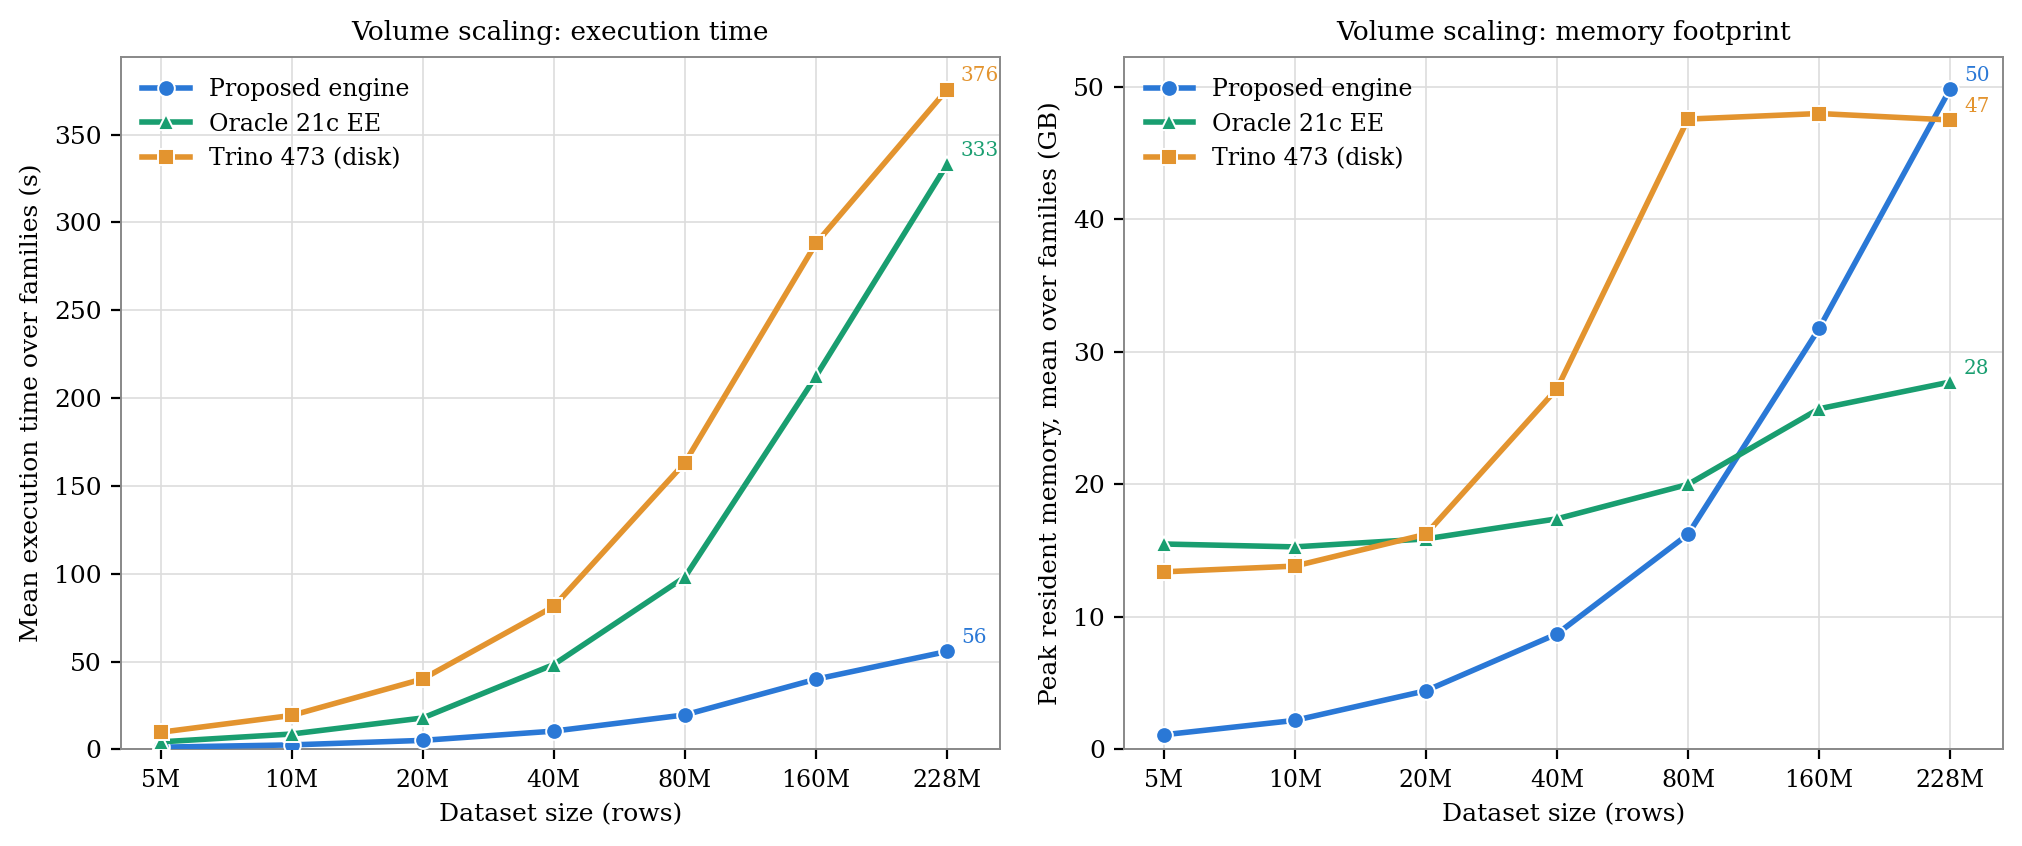
\includegraphics[width=\textwidth]{images/viz_stress_volume.png}
  \caption[Volume scaling on real data to 227.9M rows]{Volume scaling on real data: time (left) and peak memory (right).}
  \label{fig:stress_volume}
\end{figure}

Left is execution time and right is absolute peak memory.  Each size
average uses the same four families completed by all three systems at
all seven sizes.  The engine is fastest on every completed
cell, about $5.1$--$10.1\times$ ahead of Oracle~21c EE and
$11.4$--$13.8\times$
ahead of Trino on the size averages.  It also finishes the full corpus
on every pattern: 27.8\,s for \texttt{simple\_sequence}, 106.0\,s for
\texttt{complex\_nested}.  The engine and Oracle~21c EE each complete
35/35 cells.  Trino completes 33/35: \texttt{complex\_nested} crosses
the 600\,s time budget at 160\,M and 227{,}899{,}533 rows.  Because
\texttt{complex\_nested} is the slowest family for all three
systems, a mean that kept it would count it for the engine and
Oracle~21c EE at the two largest sizes but not for Trino.  Trino's
average would then omit its hardest pattern while the others kept
theirs, so the three would no longer describe the same workload, and
the composition of the mean would change along the axis.  The complete
five-family values, \texttt{complex\_nested} included, stay in
Tables~\ref{tab:stress_volume}--\ref{tab:stress_mem}.

Total resident memory tells a different story from the per-query figure
below.  The engine starts far leaner than either database: 0.7\,GB
at 5\,M rows against 13.4\,GB for Trino and 15.5\,GB for Oracle.  The
database footprints include their resident JVM or SGA baselines.  The
engine stays the leanest of the three up to 160\,M.  Only at the full corpus
does its resident data pass Oracle: 31.9\,GB against Oracle~21c EE's
27.1\,GB, still well under Trino's 42.3\,GB
(Tables~\ref{tab:stress_volume}--\ref{tab:stress_mem}).

\begin{figure}[htbp]
  \centering
  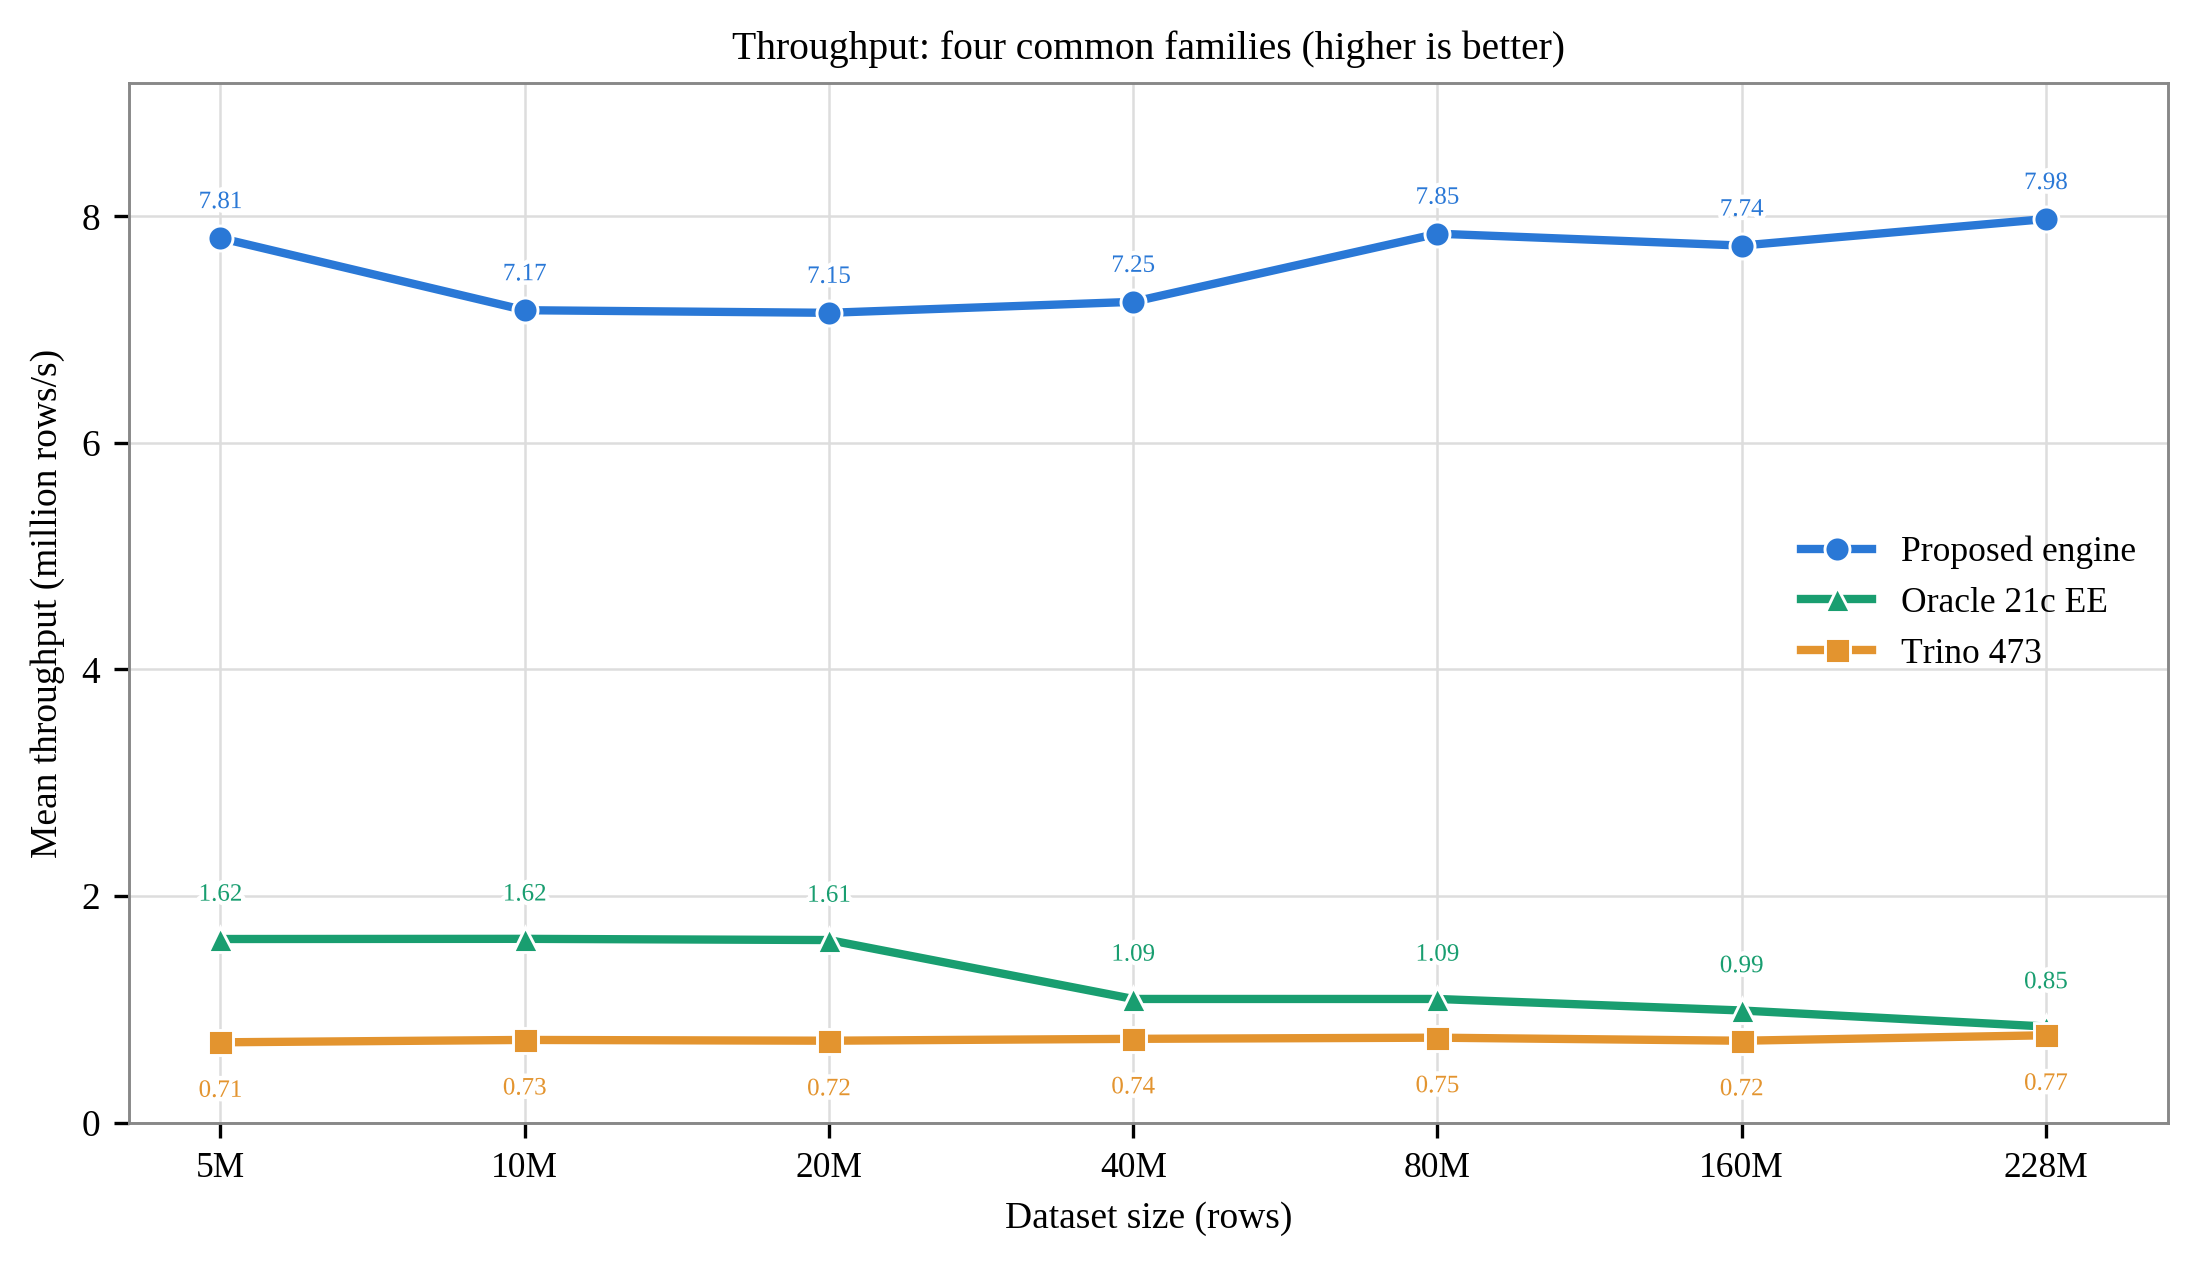
\includegraphics[width=0.82\textwidth]{images/viz_stress_throughput.png}
  \caption[Throughput scaling on real data]{Throughput scaling on real data.}
  \label{fig:stress_throughput}
\end{figure}

Figure~\ref{fig:stress_throughput} plots throughput, again averaged
over the same four common families.  The engine holds
7.1--8.0\,M\,rows/s across the whole range.
At the full size its patterns range from 2.2\,M\,rows/s on
\texttt{complex\_nested} to 9.2\,M\,rows/s on
\texttt{alternation}.  Oracle~21c EE records 0.8--1.6\,M\,rows/s
and 0.7--0.8\,M for Trino.  Oracle~21c EE drifts down as its fixed budgets
spread over more data, while Trino stays near-flat, so the two converge
at the full corpus.  The per-pattern curves remain
close to linear for all three (Figure~\ref{fig:stress_time_grid}), and every
completed cell returned identical match counts
(Tables~\ref{tab:stress_thr}, \ref{tab:stress_matches}).

\paragraph{Ranking.}
At the full corpus, the four-family average ranks the engine first,
Oracle~21c EE second, and Trino third.  The order is not the same for every
pattern.

\begin{figure}[htbp]
  \centering
  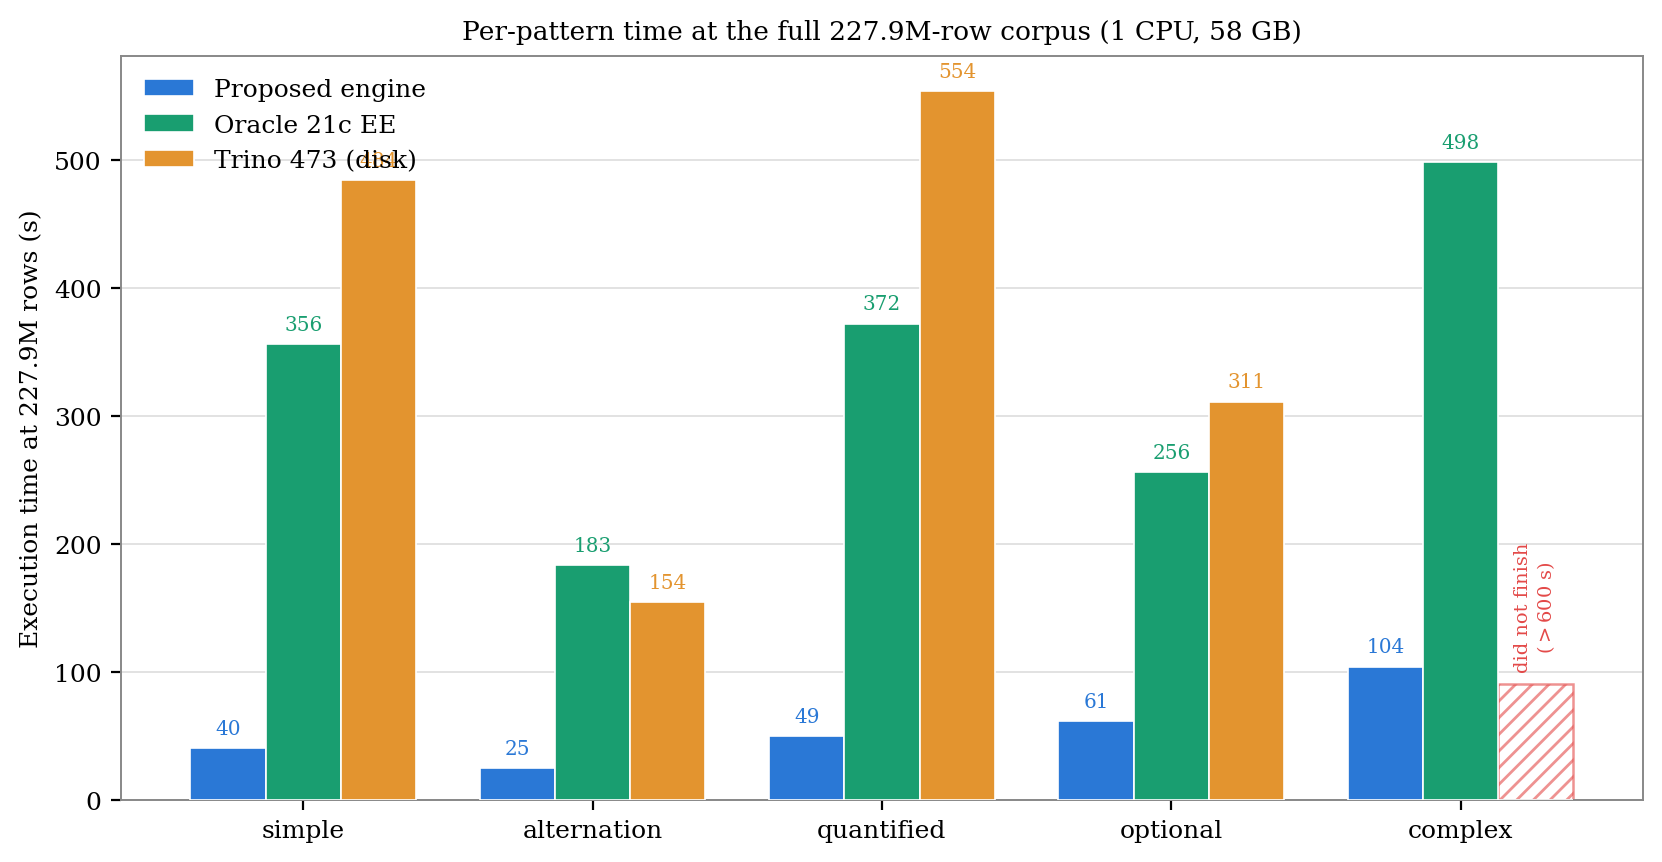
\includegraphics[width=0.92\textwidth]{images/viz_stress_patterns.png}
  \caption[Per-pattern time at the full 227.9M-row corpus]{Per-pattern
    time at the full 227.9\,M-row corpus.}
  \label{fig:stress_patterns}
\end{figure}

The engine leads on all five patterns.  Oracle~21c EE beats Trino on the
three heavy families; for \texttt{quantified}, the times are 372\,s
and 554\,s.  Oracle is also the only database to finish
\texttt{complex\_nested}, at 498\,s.  Trino wins only on the cheapest
family, \texttt{alternation}, at 154\,s versus 183\,s.  It reaches the
time wall on \texttt{complex\_nested}.  Thus the compiled engine leads,
Oracle~21c EE is the more robust database in this stress test, and Trino is
the first to reach the time wall (Table~\ref{tab:stress_volume}).

\paragraph{Memory.}
The systems trade speed for memory in opposite directions.

\begin{figure}[htbp]
  \centering
  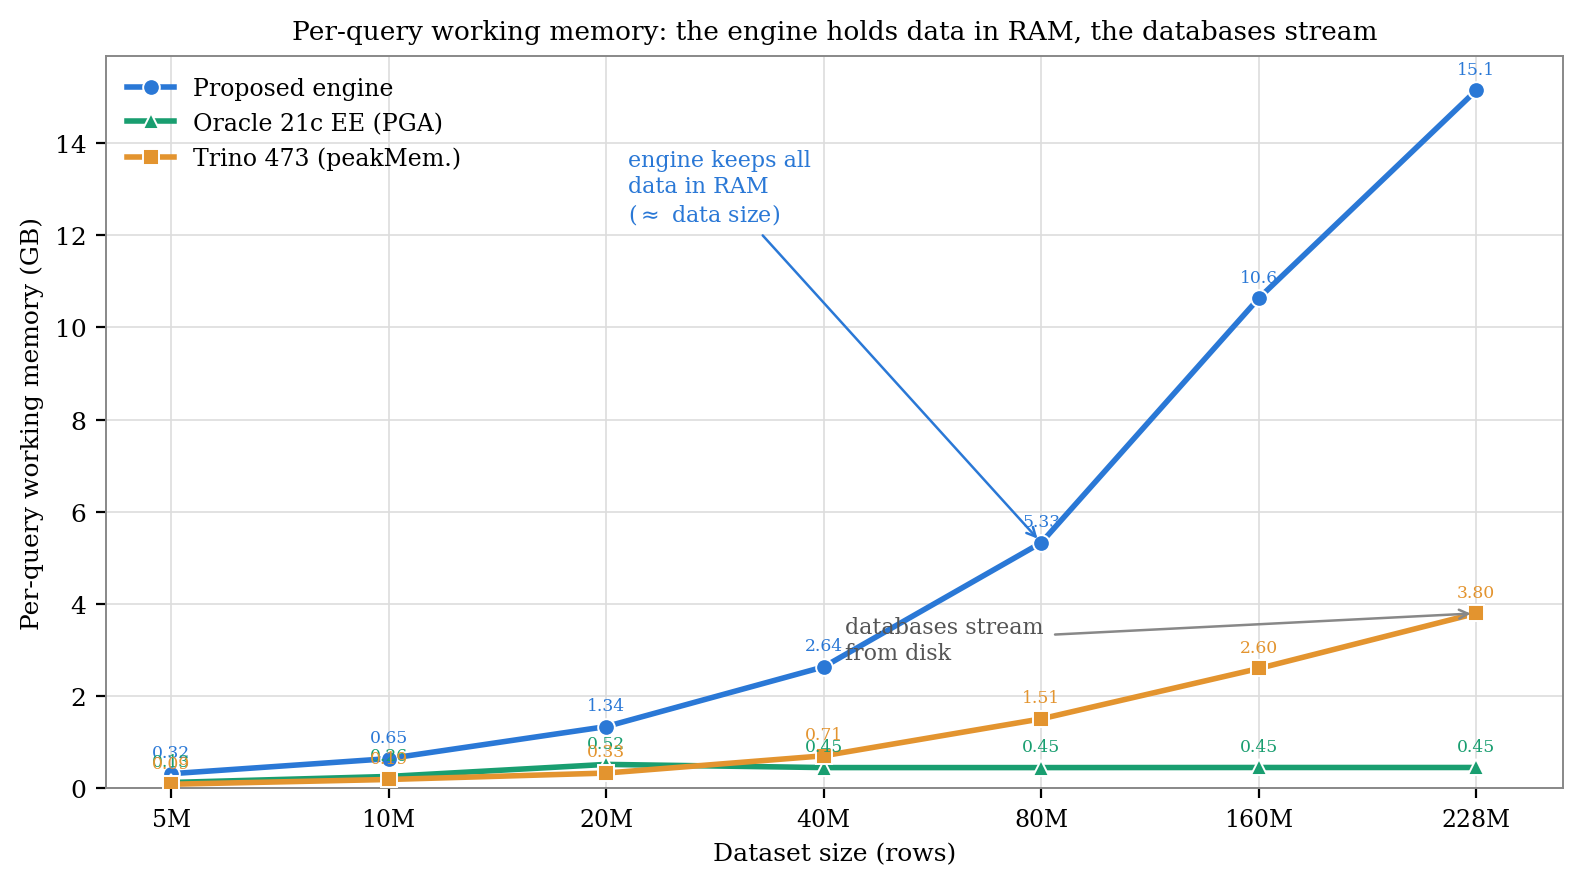
\includegraphics[width=\textwidth]{images/viz_stress_memory.png}
  \caption[Diagnostic query-memory counters on real data]{Diagnostic query-memory counters; the accounting boundaries differ.}
  \label{fig:stress_memory}
\end{figure}

Figure~\ref{fig:stress_memory} is a diagnostic view, not a
same-instrument comparison.  It places the engine's cgroup incremental
peak beside the database-native counters (Oracle PGA and Trino
\texttt{peakMemoryBytes}).  Each series is averaged over the same four
common families.  The engine reaches about 15\,GB on average and
18.5\,GB on the largest single cell at 227.9\,M rows.  Oracle stays
near 0.5\,GB and Trino below 4\,GB according to their own counters.
These counters have different accounting boundaries, so their
magnitudes should not be read as an exact memory ratio.  The
same-instrument deployment comparison is the absolute cgroup footprint
in Figure~\ref{fig:stress_volume}
(Tables~\ref{tab:stress_incmem}--\ref{tab:stress_native}).
The largest observed engine footprint was 35.7\,GB on one pattern,
below the 58\,GB limit.  The experiment does not establish an exact
maximum beyond this range.

% ................................................................
\subsection{Evaluation Validity}
\label{subsec:eval-validity}
% ................................................................

A cross-system comparison only means something if the advantage cannot
be an artifact of the measurement.  Five checks define how the results
should be read.

\emph{Correctness first.}  Times are compared only where the systems
return the same answer; every cell was checked for row-level equality
(Table~\ref{tab:cross_system_correctness}).  The 30/30 agreement is a
correctness result and a precondition for comparing execution time.

\emph{Timer scope.}  Initial data loading is excluded for all systems.
Query execution and result materialization are included, including
database result transfer to the client.  In the main matrix, five
warmups reduce cold-start and JIT effects.  The values are end-to-end
query latencies, not isolated matcher-kernel times.

\emph{Stable measurements.}  Each main-matrix cell is the IQR-filtered
mean of twenty runs.  The median coefficient of variation, the
standard deviation divided by the mean, is 3.5\% (engine), 2.3\%
(Oracle), and 3.8\% (Trino).  The stress test uses fewer runs per cell,
five after two warmups, but varies less: its median coefficient of
variation is at most 1.0\% for the three systems.  This supports the
stability of both sets of means.

\emph{Separate campaigns.}  The systems used the same host, logical
queries, input rows, CPU allocation, and outer memory limit, but they
were measured one after another rather than side by side.  Every
campaign ran on one CPU core, each with its own repetition count.  The
main benchmark uses five warmups and twenty measured runs per cell,
under a 32\,GB limit with resident inputs.  The stress study uses two
warmups and five runs, under 58\,GB with system-appropriate scalable
storage.  The ordering test repeats the main protocol.  The
state-dependent case keeps twenty runs for the engine but two for the
retained database values.  No figure here comes from a concurrent
head-to-head run.

\emph{Narrow scope.}  The claim is only that the engine is faster
\emph{on this workload} (one partition, in-memory input, the supported
subset) on one machine.  The systems had the same outer CPU and
memory limits in the main matrix.  Their execution models and measured process
boundaries also differ.  Database tuning could change the gap.

% ................................................................
\subsection{Key Findings}
\label{subsec:eval-findings}
% ................................................................

The main findings are as follows.

\emph{Speed.}  The engine was fastest on all 30 cross-system cells, and
it stayed $5.1$--$10.1\times$ ahead of Oracle~21c EE and
$11.4$--$13.8\times$ ahead of Trino on the four common stress-test
families to 227.9\,M rows.

\emph{Why it is faster on this workload.}  The engine is specialized
for in-process DataFrame matching.  It avoids database planning,
catalog, transaction, client-protocol, and data-transfer costs.  Its
compiler turns supported predicates into column operations and
integer-code comparisons, then uses decision tables and grouped NumPy
reductions to reduce per-row Python work.  Ordered input also lets it
skip sorting, although Section~\ref{subsec:eval-ordering} shows that
it remains fastest when sorting is forced.  This advantage applies to
the supported single-node workload, not to every pattern or deployment.

\emph{Correctness.}  All 30 main pattern--size combinations matched
across the three systems.  Every completed stress database cell also
matched the engine.  The engine and Oracle completed 35/35 stress
cells; Trino completed 33/35.

\emph{Scalability.}  Execution time was close to linear for all three
systems over the tested range.  The engine's measured memory was also
close to linear, and it finished the full 227.9\,M-row corpus.  It did
not reach an internal size or memory limit; RAM remains the likely
boundary for larger in-memory inputs.  Oracle~21c EE also reached the full
size; Trino's hardest pattern exceeded the time budget at 160\,M and
227.9\,M rows.

\emph{The trade-off.}  The engine keeps its DataFrame in RAM and builds
whole-column working arrays.  The input is already part of the memory
baseline, while the incremental peak measures additional query-time
growth.  Its total footprint is lower than
the resident database containers in the main benchmark, but that
relationship reverses against Oracle at the largest stress-test size.

\emph{Honest limits.}  The lead is bounded by what the compiler can
turn into column operations.  The state-dependent \texttt{DEFINE} that
once made both databases faster now uses a compiled incremental plan.
This solves one aggregate form, not the full class.
Other state-dependent or ambiguous forms can still use the generic
exact evaluator and may reach its explicit work limit.  At scale, the
resident DataFrame makes RAM a likely boundary.  The study maps where
each system's usable region lies; it does not crown a universal winner.

% ----------------------------------------------------------------
\section{Chapter Summary}
\label{sec:eval-summary}
% ----------------------------------------------------------------

This chapter evaluated correctness, coverage, complexity, usability,
performance, scalability, and memory.  All three systems agreed in the
30 main pattern--size combinations, and every completed stress database
cell matched the engine.  The engine and Oracle completed all 35 stress
cells; Trino completed 33.  The engine recorded the lowest time on the
evaluated workload and scaled close to linearly, while its query-time
memory grew with the input.  These findings apply to the supported
single-node workload and stated resource limits.  The next chapter
summarizes the contributions, limitations, and future work.
